\pdfpagewidth = 8.5in
\pdfpageheight = 11.0in
\usepackage[left=1in,right=1in,top=1in,bottom=1in]{geometry}

\pagestyle{plain}
\pagenumbering{arabic}
\usepackage{setspace}
\usepackage[usenames]{color}
\usepackage[fleqn]{amsmath}
\usepackage{amssymb}
\usepackage{graphicx}
\usepackage{url}
\usepackage{verbatim}
\usepackage{appendix}
\usepackage{indentfirst}
\usepackage{booktabs}
\usepackage{multirow}
\usepackage[table, x11names]{xcolor}
\usepackage{ragged2e}
\usepackage{upgreek}
\usepackage{lscape}
\usepackage{longtable}
\usepackage[flushleft, referable]{threeparttablex}
\usepackage{rotating}
\usepackage[T1]{fontenc}
\usepackage[titles]{tocloft}
\usepackage{xspace}
\usepackage{ifthen}
\usepackage{cancel}
\usepackage{rotating}
\usepackage{array}
\usepackage{tabulary}
\usepackage{authblk}

\usepackage{hyperref}
\hypersetup{pdfborder={0 0 0}, colorlinks=true, urlcolor=black, linkcolor=black, citecolor=black}
\usepackage[capitalize]{cleveref}
\newcommand{\crefrangeconjunction}{--}

\usepackage[right, mathlines]{lineno}
\setlength\linenumbersep{1cm}
\def\linenumberfont{\normalfont\scriptsize\sffamily}

% \usepackage[format=plain, labelsep=period, justification=raggedright, singlelinecheck=true, skip=2pt, font=sf]{caption}
\usepackage{caption}
\DeclareCaptionLabelFormat{noSpace}{{#1}{#2}}
\DeclareCaptionListFormat{figList}{Figure {#2}.}
\DeclareCaptionListFormat{sFigList}{Figure S{#2}.}
\usepackage{subfig}

%\DeclareMathSizes{12}{12}{7}{5}

% \usepackage[round]{natbib}

% \makeatletter
%   \renewcommand{\section}{\@startsection{section}{1}{0mm}%
%     {-12pt}%
%     {12pt}%
%     {\sffamily\LARGE\itshape}}
% \makeatother

% \makeatletter
%   \renewcommand{\subsection}{\@startsection{subsection}{1}{0mm}%
%   {-10pt}%
%   {4pt}%
%   {\sffamily\large\bfseries\MakeUppercase}}
% \makeatother

% \makeatletter
%   \renewcommand{\subsubsection}{\@startsection{subsubsection}{1}{0mm}%
%   {-10pt}%
%   {10pt}%
%   {\sffamily\large\itshape}}
% \makeatother

% make list of figures ragged right
% \makeatletter
%   \renewcommand{\@tocrmarg}{0cm plus1fil}
% \makeatother

\setlength\linenumbersep{1cm}

% \newcommand{\change}[1]{{\color{blue} #1}\xspace}
\newcommand{\change}[1]{{\color{black} #1}\xspace}


\newcommand{\citationNeeded}{\textcolor{magenta}{\textbf{[CITATION NEEDED!]}}\xspace}
\newcommand{\tableNeeded}{\textcolor{magenta}{\textbf{[TABLE NEEDED!]}}\xspace}
\newcommand{\figureNeeded}{\textcolor{magenta}{\textbf{[FIGURE NEEDED!]}}\xspace}
\newcommand{\highLight}[1]{\textcolor{magenta}{\MakeUppercase{#1}}}

\newcommand{\editorialNote}[1]{\textcolor{red}{[\textit{#1}]}}
\newcommand{\ignore}[1]{}
\newcommand{\addTail}[1]{\textit{#1}.---}
\newcommand{\super}[1]{\ensuremath{^{\textrm{#1}}}}
\newcommand{\sub}[1]{\ensuremath{_{\textrm{#1}}}}
\newcommand{\dC}{\ensuremath{^\circ{\textrm{C}}}}

\providecommand{\e}[1]{\ensuremath{\times 10^{#1}}}

\newcommand{\mthnote}[2]{{\color{red} #2}\xspace}
\newcommand{\cwlnote}[2]{{\color{orange} #2}\xspace}

\newcommand{\ifTwoArgs}[3]{\ifthenelse{\equal{#1}{}\or\equal{#2}{}}{}{#3}\xspace}
\newcommand{\ifArg}[2]{\ifthenelse{\equal{#1}{}}{}{#2}\xspace}

%% New notation for divergence times
\newcommand{\divTime}[1]{\ensuremath{\tau_{#1}}\xspace}
\newcommand{\divTimeVector}{\ensuremath{\boldsymbol{\divTime{}}}\xspace}
\newcommand{\divTimeIndex}[1]{\ensuremath{t_{#1}}\xspace}
\newcommand{\divTimeIndexVector}{\ensuremath{\mathbf{\divTimeIndex{}}}\xspace}
\newcommand{\divTimeMap}[1]{\ensuremath{T_{#1}}\xspace}
\newcommand{\divTimeMapVector}{\ensuremath{\mathbf{\divTimeMap{}}}\xspace}
\newcommand{\divTimeScaled}[2]{\ensuremath{\mathcal{T}_{#1\protect\ifTwoArgs{#1}{#2}{,}#2}}\xspace}
\newcommand{\divTimeScaledVector}{\ensuremath{\mathbf{\divTimeScaled{}{}}}\xspace}
\newcommand{\divTimeMean}{\ensuremath{\bar{\divTimeMap{}}}\xspace}
\newcommand{\divTimeVar}{\ensuremath{s^{2}_{\divTimeMap{}}}\xspace}
\newcommand{\divTimeDispersion}{\ensuremath{D_{\divTimeMap{}}}\xspace}
\newcommand{\divTimeNum}{\ensuremath{\lvert \divTimeVector \rvert}\xspace}
\newcommand{\demographicParams}[1]{\ensuremath{\Theta_{#1}}\xspace}
\newcommand{\demographicParamVector}{\ensuremath{\mathbf{\demographicParams{}}}\xspace}
\newcommand{\popSampleSize}[2]{\ensuremath{n_{#1\protect\ifTwoArgs{#1}{#2}{,}#2}}}
\newcommand{\gammaShape}[1]{\ensuremath{a_{#1}}\xspace}
\newcommand{\gammaScale}[1]{\ensuremath{b_{#1}}\xspace}
\newcommand{\betaA}[1]{\ensuremath{a_{#1}}\xspace}
\newcommand{\betaB}[1]{\ensuremath{b_{#1}}\xspace}
\newcommand{\integerPartitionSet}[1]{\ensuremath{a({#1})}\xspace}
\newcommand{\integerPartitionNum}[1]{\ensuremath{\lvert \integerPartitionSet{#1} \rvert}\xspace}
\newcommand{\concentrationParam}{\ensuremath{\chi}\xspace}
\newcommand{\stirlingFirst}[2]{\ensuremath{c(#1, #2)}\xspace}
\newcommand{\descendantThetaMean}[1]{\ensuremath{\bar{\theta}_{D\protect\ifArg{#1}{,}#1}}\xspace}
\newcommand{\numPriorSamples}{\ensuremath{\mathbf{n}}\xspace}
\newcommand{\paramSampleVector}[1]{\ensuremath{\Lambda_{#1}}\xspace}
\newcommand{\paramSampleMatrix}{\ensuremath{\boldsymbol{\paramSampleVector{}}}\xspace}
\newcommand{\modelDPP}{\ensuremath{M_{DPP}}\xspace}
\newcommand{\modelDPPOrdered}{\ensuremath{M^{\circ}_{DPP}}\xspace}
\newcommand{\modelUniform}{\ensuremath{M_{Uniform}}\xspace}
\newcommand{\modelUshaped}{\ensuremath{M_{Ushaped}}\xspace}
\newcommand{\modelOld}{\ensuremath{M_{msBayes}}\xspace}
\newcommand{\priorDPP}[1]{\ensuremath{DP(\concentrationParam #1)}\xspace}
\newcommand{\priorUniform}{\ensuremath{DU\{\integerPartitionSet{\npairs{}}\}}\xspace}
\newcommand{\priorOld}{\ensuremath{DU\{1, \ldots, \npairs{}\}}\xspace}
\newcommand{\powerSeriesOld}{\ensuremath{\mathcal{M}_{msBayes}}\xspace}
\newcommand{\powerSeriesUniform}{\ensuremath{\mathcal{M}_{Uniform}}\xspace}
\newcommand{\powerSeriesExp}{\ensuremath{\mathcal{M}_{Exp}}\xspace}

\newcommand{\allDatasets}{\ensuremath{\mathcal{\alignment{}{}}}\xspace}
\newcommand{\allParameterValues}{\ensuremath{\boldsymbol{\Theta}}\xspace}
\newcommand{\bayesfactor}[2]{\ensuremath{BF_{#1\protect\ifArg{#2}{,}#2}}}
\newcommand{\given}{\ensuremath{\,|\,}\xspace}
\newcommand{\msb}{\upshape\texttt{\MakeLowercase{ms\MakeUppercase{B}ayes}}\xspace}
\newcommand{\abctoolbox}{\upshape\texttt{ABCtoolbox}\xspace}
\newcommand{\dppmsbayes}{\upshape\texttt{dpp-msbayes}\xspace}
\newcommand{\pymsbayes}{\upshape\texttt{PyMsBayes}\xspace}
\newcommand{\hky}{HKY85\xspace}
\newcommand{\uniformMin}[1]{\ensuremath{a_{#1}}\xspace}
\newcommand{\uniformMax}[1]{\ensuremath{b_{#1}}\xspace}
\newcommand{\locusRateHetShapeParameter}{\ensuremath{\alpha}\xspace}
\newcommand{\ancestralThetaVector}{\ensuremath{\boldsymbol{\theta_{A}}}\xspace}
\newcommand{\descendantThetaVector}[1]{\ensuremath{\boldsymbol{\theta_{D#1}}}\xspace}
\newcommand{\divtscaledvector}{\ensuremath{\mathbf{{\divtscaled{}{}}}}\xspace}
\newcommand{\divtvector}{\ensuremath{\boldsymbol{\divt{}}}\xspace}
\newcommand{\divtuniquevector}{\ensuremath{\mathbf{\divtunique{}}}\xspace}
\newcommand{\bottleTimeVector}{\ensuremath{\boldsymbol{\bottleTime{}}}\xspace}
\newcommand{\bottleTime}[1]{\ensuremath{\divt{B\ifArg{#1}{,}#1}}\xspace}
\newcommand{\bottleScalarVector}[1]{\ensuremath{\boldsymbol{\bottleScalar{#1}{}}}\xspace}
\newcommand{\bottleScalar}[2]{\ensuremath{\zeta_{D#1\protect\ifArg{#2}{,}#2}}\xspace}
\newcommand{\migrationRateVector}{\ensuremath{\mathbf{\migrationRate{}}}\xspace}
\newcommand{\geneTreeVector}{\ensuremath{\mathbf{\geneTree{}{}}}\xspace}
\newcommand{\alignmentVector}{\ensuremath{\mathbf{\alignment{}{}}}\xspace}
\newcommand{\alignment}[2]{\ensuremath{X_{#1\protect\ifTwoArgs{#1}{#2}{,}#2}}\xspace}
\newcommand{\geneTree}[2]{\ensuremath{G_{#1\protect\ifTwoArgs{#1}{#2}{,}#2}}\xspace}
\newcommand{\migrationRate}[1]{\ensuremath{m_{#1}}\xspace}
\newcommand{\recombinationRate}{\ensuremath{r}\xspace}
\newcommand{\ploidyScalar}[2]{\ensuremath{\rho_{#1\protect\ifTwoArgs{#1}{#2}{,}#2}}\xspace}
\newcommand{\ploidyScalarVector}{\ensuremath{\boldsymbol{\ploidyScalar{}{}}}\xspace}
\newcommand{\descendantRelativeThetaVector}[1]{\ensuremath{\boldsymbol{\eta_{D#1}}}\xspace}
\newcommand{\descendantRelativeTheta}[2]{\ensuremath{\eta_{D#1\protect\ifArg{#2}{,}#2}}\xspace}
\newcommand{\mutationRateScalarConstant}[2]{\ensuremath{\nu_{#1\protect\ifTwoArgs{#1}{#2}{,}#2}}\xspace}
\newcommand{\mutationRateScalarConstantVector}{\ensuremath{\boldsymbol{\mutationRateScalarConstant{}{}}}\xspace}
\newcommand{\locusMutationRateScalar}[1]{\ensuremath{\upsilon_{#1}}\xspace}
\newcommand{\locusMutationRateScalarVector}{\ensuremath{\boldsymbol{\upsilon}}\xspace}
\newcommand{\hkyModel}[2]{\ensuremath{\phi_{#1\protect\ifTwoArgs{#1}{#2}{,}#2}}\xspace}
\newcommand{\hkyModelVector}{\ensuremath{\boldsymbol{\hkyModel{}{}}}\xspace}
\newcommand{\mutationRate}{\ensuremath{\mu}\xspace}
\newcommand{\iid}{\textit{iid}\xspace}
\newcommand{\model}[1]{\ensuremath{\Theta}\xspace}
\newcommand{\npairs}[1]{\ensuremath{Y_{#1}}}
\newcommand{\nloci}[1]{\ensuremath{k_{#1}}\xspace}
\newcommand{\nlociTotal}{\ensuremath{K}\xspace}
\newcommand{\myTheta}[1]{\ensuremath{\theta_{#1}}}
\newcommand{\ancestralTheta}[1]{\ensuremath{\theta_{A\protect\ifArg{#1}{,}#1}}\xspace}
\newcommand{\descendantTheta}[2]{\ensuremath{\theta_{D#1\protect\ifArg{#2}{,}#2}}\xspace}
\newcommand{\meanDescendantTheta}[1]{\ensuremath{\descendantTheta{}{#1}}\xspace}
\newcommand{\nucdiv}[1]{\ensuremath{\pi_{#1}}}

\newcommand{\ssVector}[1]{\ensuremath{\mathbf{\alignmentSS{#1}{}}}\xspace}
\newcommand{\ssVectorObs}{\ensuremath{\ssVector{}^*}\xspace}
\newcommand{\ssSpace}{\ensuremath{\euclideanSpace{\ssVectorObs}}\xspace}
\newcommand{\ssVectorObsPLS}{\ensuremath{\ssVectorObs_{PLS}}\xspace}
\newcommand{\alignmentSS}[2]{\ensuremath{S_{#1\protect\ifTwoArgs{#1}{#2}{,}#2}}\xspace}
\newcommand{\alignmentSSObs}[2]{\ensuremath{\alignmentSS{#1}{#2}^*}\xspace}
\newcommand{\tol}{\ensuremath{\epsilon}\xspace}
\newcommand{\euclideanSpace}[1]{\ensuremath{B_{\tol}(#1)}\xspace}
\newcommand{\hpvector}[1]{\ensuremath{\Lambda_{#1}}}
\newcommand{\divtscaled}[2]{\ensuremath{t_{#1\protect\ifTwoArgs{#1}{#2}{,}#2}}}
\newcommand{\divt}[1]{\ensuremath{\tau_{#1}}}
\newcommand{\divtunique}[1]{\ensuremath{T_{#1}}}
\newcommand{\ssMatrix}{\ensuremath{\mathbb \alignmentSS{}{}}\xspace}
\newcommand{\ssMatrixRaw}[1]{\ensuremath{{\ssMatrix}_{stats#1}}\xspace}
\newcommand{\ssMatrixPLS}[1]{\ensuremath{{\ssMatrix}_{PLS#1}}\xspace}
\newcommand{\hpmatrix}[1]{\ensuremath{\mathcal{P}_{#1}}}
\newcommand{\meant}[2]{\ensuremath{E(\divt{#1})_{#2}}}
\newcommand{\meantestimate}{\ensuremath{\hat{E(\divt{})}}\xspace}
\newcommand{\vart}[2]{\ensuremath{Var(\divt{#1}{})_{#2}}}
\newcommand{\vmratio}[1]{\ensuremath{\Omega_{#1}}}
\newcommand{\numt}[1]{\ensuremath{\Psi_{#1}}}
\newcommand{\probnumt}[2]{\ensuremath{p(\numt{#1} = {#2})}}
\newcommand{\postprobnumt}[1]{\ensuremath{p(\numt{} = {#1}|\ssSpace)}}
\newcommand{\postprobnumtnot}[1]{\ensuremath{p(\numt{} \neq {#1}|\ssSpace)}}
\newcommand{\postprobomegasimult}{\ensuremath{p(\vmratio{} < 0.01 | \ssSpace)}\xspace}
\newcommand{\modelprior}[1]{\ensuremath{f(\model{})}}
\newcommand{\modelpost}[1]{\ensuremath{f(\model{}|\ssSpace)}}
\newcommand{\npriorsamples}{\ensuremath{n}\xspace}
\newcommand{\globalcoalunit}{\ensuremath{4\globalpopsize}\xspace}
\newcommand{\globalpopsize}{\ensuremath{N_C}\xspace}
\newcommand{\effectivePopSize}[1]{\ensuremath{N_e{#1}}\xspace}
\newcommand{\coalunit}{\ensuremath{4\effectivePopSize{}}\xspace}
\newcommand{\priorsample}[1]{\ensuremath{\hpmatrix{\modelprior{}}}}
\newcommand{\truncprior}[1]{\ensuremath{\hpmatrix{\tol}}\xspace}
\newcommand{\postsample}[1]{\ensuremath{\hpmatrix{\modelpost{}}}}
\newcommand{\abcllr}[1]{ABC\sub{LLR}}
\newcommand{\abcglm}[1]{ABC\sub{GLM}}
\newcommand{\integerPartition}[1]{\ensuremath{a({#1})}}
\newcommand{\uniqueModel}[2]{\ensuremath{M_{#1\protect\ifTwoArgs{#1}{#2}{,}#2}}}
\newcommand{\taxonLocusVector}[1]{\ensuremath{\{#1{1}{1},\ldots,#1{\npairs{}}{\nloci{\npairs{}}}\}}\xspace}
\newcommand{\taxonVector}[1]{\ensuremath{\{#1{1},\ldots,#1{\npairs{}}\}}\xspace}
\newcommand{\locusVector}[1]{\ensuremath{\{#1{1},\ldots,#1{\nlociTotal}\}}\xspace}

\newcommand{\validationAccuracyCaption}[2]{Estimation accuracy for model
    #2 when analyzing data generated under #1.
    A random sample of 5000 posterior estimates (from 50,000) are plotted,
    including both (A, B, \& C) unadjusted and (D, E, \&
    F) GLM-regression-adjusted estimates.
    Normal random variates ($N(0, 0.005)$) have been added to the estimates and
    true values of \divTimeNum (A \& D) to reduce overlap of plot symbols.
    The root mean square error (RMSE) calculated from the 5000 estimates is
    provided.}
\newcommand{\validationModelChoiceCaption}[2]{Model-choice accuracy for model
    #2 when analyzing data generated under #1.
    The estimated posterior probability of a single divergence event, based on
    (A \& C) $\divTimeNum = 1$ and (B \& D) $\divTimeDispersion < 0.01$, from
    50,000 posterior estimates are assigned to bins of width 0.05 and plotted
    against the proportion of replicates in each bin where the truth is
    $\divTimeNum = 1$ or $\divTimeDispersion < 0.01$.
    Results based on the (A \& B) unadjusted and (C \& D) GLM-adjusted
    posterior estimates are shown.}
\newcommand{\powerAccuracyCaption}[2]{Estimation accuracy for model
    #2 when analyzing data generated under the series of models #1.
    The true versus estimated value of the dispersion index of divergence
    times (\divTimeDispersion) is plotted for 1000 datasets simulated
    under each of the #1 models, and the proportion of estimates less
    than the truth, $p(\hat{\divTimeDispersion} < \divTimeDispersion)$,
    is shown for each data model.}
\newcommand{\powerPsiCaption}[2]{
    The power of model #2 to detect random variation in divergence times as
    simulated under the series of models #1.
    The plots illustrate the estimated number of divergence events
    ($\hat{\divTimeNum}$) from analyses of 1000 datasets simulated under each
    of the #1 models, with the the estimated probability of the model inferring
    one divergence event, $p(\hat{\divTimeNum} = 1)$, given for each data
    model.}
\newcommand{\powerDispersionCaption}[2]{
    The power of model #2 to detect random variation in divergence times as
    simulated under the series of models #1.
    The plots illustrate the estimated dispersion index of divergence times
    ($\hat{\divTimeDispersion}$) from analyses of 1000 datasets simulated under
    each of the #1 models, with the the estimated probability of the model
    inferring one divergence event, $p(\hat{\divTimeDispersion} < 0.01)$, given
    for each data model.}
\newcommand{\powerPsiProbCaption}[2]{
    The tendency of model #2 to support one divergence event when there is
    random variation in divergence times as simulated under the series of
    models #1.
    The plots illustrate histograms of the estimated posterior probability of
    the one divergence model, $p(\divTimeNum = 1 | \ssSpace)$, from analyses of
    1000 datasets simulated under each of the #1 models, with the the estimated
    probability of the model strongly supporting one divergence event,
    $p(BF_{\divTimeNum = 1, \divTimeNum \neq 1} > 10)$, given for each data
    model.}
\newcommand{\powerDispersionProbCaption}[2]{
    The tendency of model #2 to support one divergence event when there is
    random variation in divergence times as simulated under the series of
    models #1.
    The plots illustrate histograms of the estimated posterior probability of
    the one divergence model, $p(\divTimeDispersion < 0.01 | \ssSpace)$, from
    analyses of 1000 datasets simulated under each of the #1 models, with the
    the estimated probability of the model strongly supporting one divergence
    event, $p(BF_{\divTimeDispersion < 0.01, \divTimeDispersion \geq 0.01} >
    10)$, given for each data model.}
\newcommand{\simulationDescription}[2]{\change{Each plot represents #1
    simulation replicates using the same $#2$ samples from the prior}}
\newcommand{\simulationDistribution}{\ensuremath{\divt{} \sim U(0,
    \divt{max})}\xspace}
\newcommand{\estimateDescription}[2]{All estimates were obtained using #1 and #2}
\newcommand{\estimateDescriptionUncorrected}[1]{All estimates based on
    unadjusted posterior, \truncprior{}, obtained using #1}
\newcommand{\priorDescription}[4]{Prior settings were \priorSettings{#1}{#2}{#3}{#4}}
\newcommand{\priorSettings}[4]{$\divt{} \sim U(0, #1)$,
    $\meanDescendantTheta{} \sim U(#2, #3)$, and
    $\ancestralTheta{}{} \sim U(#2, #4)$}
\newcommand{\priorDescriptionBug}[4]{Prior settings were
    \priorSettingsBug{#1}{#2}{#3}{#4}}
\newcommand{\priorSettingsBug}[4]{$\divt{} \sim U(0, #1)$,
    $\meanDescendantTheta{} \sim U(#2, #3)$, and
    $\ancestralTheta{}{} \sim U(0.01, #4)$}
\newcommand{\simulationScheme}{simulations where \divt{} (in \globalcoalunit
    generations) for 22 population pairs is drawn from a series of uniform
    distributions, \simulationDistribution}
\newcommand{\captionPowerOmega}{Histograms of the estimated dispersion index
    of divergence times ($\hat{\vmratio{}}$) from \simulationScheme.
    The threshold for one divergence event \citep{Hickerson2006} is indicated
    by the dashed line, and the estimated probability of inferring one
    divergence event, $p(\hat{\vmratio{}}\le 0.01)$, is given for each
    \divt{max}}
\newcommand{\captionPowerPsiMode}{Histograms of the estimated number of
    divergence events ($\hat{\numt{}}$) from \simulationScheme.
    The estimated probability of inferring one divergence event,
    $p(\hat{\numt{}} = 1)$, is given for each \divt{max}}
\newcommand{\captionPowerPsi}{Histograms of the estimated posterior
    probability of one divergence event, \postprobnumt{1}, from
    \simulationScheme.
    The estimated probability of inferring one divergence event with a
    Bayes factor greater than 10 (dashed black line),
    $p(\bayesfactor{\numt{}=1}{\numt{} \ne 1} > 10)$, is given for each \divt{max}.
    The red line indicates $\postprobnumt{1} = 0.95$, and the estimated
    probability of inferring a posterior probability greater than 0.95 is given
    to the right of the line.}
\newcommand{\captionAccuracy}[1]{Accuracy and precision of #1 estimates from
    \simulationScheme.
    The proportion of estimates less than the true value ($p(\hat{#1}<#1)$) is
    given for each \divt{max}}
\newcommand{\samplingErrorTableNote}{An estimate of 1.0 for a posterior probability
    is an artifact of sampling error}


\newcommand{\refAccuracyALL}[1]{\labelcref{fig_acc_t_ss_llr_bug,fig_acc_t_ss_glm_bug,fig_acc_t_pls_llr_bug,fig_acc_t_pls_glm_bug,fig_acc_o_ss_llr_bug,fig_acc_o_ss_glm_bug,fig_acc_o_pls_llr_bug,fig_acc_o_pls_glm_bug}}
\newcommand{\refAccuracySS}[1]{\labelcref{fig_acc_t_ss_llr_bug,fig_acc_t_ss_glm_bug,fig_acc_o_ss_llr_bug,fig_acc_o_ss_glm_bug}}
\newcommand{\refAccuracySSfull}[1]{\labelcref{fig_acc_t_ssfull_llr_bug,fig_acc_t_ssfull_glm_bug,fig_acc_o_ssfull_llr_bug,fig_acc_o_ssfull_glm_bug}}
\newcommand{\refSSfull}[1]{\labelcref{fig_acc_t_ssfull_llr_bug,fig_acc_t_ssfull_glm_bug,fig_acc_o_ssfull_llr_bug,fig_acc_o_ssfull_glm_bug,fig_pow_o_ssfull_llr_bug,fig_pow_o_ssfull_glm_bug,fig_pow_psi_modes_ssfull_glm_bug}}
\newcommand{\refSS}[1]{\labelcref{fig_acc_t_ss_llr_bug,fig_acc_t_ss_glm_bug,fig_acc_o_ss_llr_bug,fig_acc_o_ss_glm_bug,fig_pow_o_ss_llr_bug,fig_pow_o_ss_glm_bug,fig_pow_psi_ss}}
\newcommand{\refAccuracyPLS}[1]{\labelcref{fig_acc_t_pls_llr_bug,fig_acc_t_pls_glm_bug,fig_acc_o_pls_llr_bug,fig_acc_o_pls_glm_bug}}
\newcommand{\refAccuracySScorrected}[1]{\labelcref{fig_acc_t_ss_llr_bug,fig_acc_t_ss_glm_bug,fig_acc_o_ss_llr_bug,fig_acc_o_ss_glm_bug}}
\newcommand{\refAccuracyPLScorrected}[1]{\labelcref{fig_acc_t_pls_llr_bug,fig_acc_t_pls_glm_bug,fig_acc_o_pls_llr_bug,fig_acc_o_pls_glm_bug}}
\newcommand{\refAccuracyUncorrected}[1]{\labelcref{fig_acc_t_ss_unc,fig_acc_t_pls_unc,fig_acc_o_ss_unc,fig_acc_o_pls_unc}}
\newcommand{\refAccuracyCorrected}[1]{\labelcref{fig_acc_t_ss_llr_bug,fig_acc_t_ss_glm_bug,fig_acc_t_pls_llr_bug,fig_acc_t_pls_glm_bug,fig_acc_o_ss_llr_bug,fig_acc_o_ss_glm_bug,fig_acc_o_pls_llr_bug,fig_acc_o_pls_glm_bug}}
\newcommand{\refAccuracyGLM}[1]{\labelcref{fig_acc_t_ss_glm_bug,fig_acc_t_pls_glm_bug,fig_acc_o_ss_glm_bug,fig_acc_o_pls_glm_bug}}
\newcommand{\refAccuracyLLR}[1]{\labelcref{fig_acc_t_ss_llr_bug,fig_acc_t_pls_llr_bug,fig_acc_o_ss_llr_bug,fig_acc_o_pls_llr_bug}}
\newcommand{\refAccuracyOmega}[1]{\labelcref{fig_acc_o_ss_llr_bug,fig_acc_o_ss_glm_bug,fig_acc_o_pls_llr_bug,fig_acc_o_pls_glm_bug}}
\newcommand{\refAccuracyOmegaUncorrected}[1]{\labelcref{fig_acc_o_ss_unc,fig_acc_o_pls_unc}}
\newcommand{\refAccuracyOmegaCorrected}[1]{\labelcref{fig_acc_o_ss_llr_bug,fig_acc_o_ss_glm_bug,fig_acc_o_pls_llr_bug,fig_acc_o_pls_glm_bug}}
\newcommand{\refAccuracyTime}[1]{\labelcref{fig_acc_t_ss_llr_bug,fig_acc_t_ss_glm_bug,fig_acc_t_pls_llr_bug,fig_acc_t_pls_glm_bug}}

\newcommand{\tn}{\tabularnewline}

\newcommand{\widthFigure}[5]{\begin{figure}[htbp]
\begin{center}
    \includegraphics[width=#1\textwidth]{#2}
    \captionsetup{#3}
    \caption{#4}
    \label{#5}
    \end{center}
    \end{figure}}

\newcommand{\heightFigure}[5]{\begin{figure}[htbp]
\begin{center}
    \includegraphics[height=#1]{#2}
    \captionsetup{#3}
    \caption{#4}
    \label{#5}
    \end{center}
    \end{figure}}

\newcommand{\mFigure}[3]{\widthFigure{1.0}{#1}{listformat=figList}{#2}{#3}\clearpage}
\newcommand{\siFigure}[3]{\widthFigure{1.0}{#1}{name=Figure S, labelformat=noSpace, listformat=sFigList}{#2}{#3}\clearpage}


\newcommand{\allParameters}[1]{\ensuremath{\theta_{#1}}\xspace}
\bibliography{../../manuscripts/bib/references}

% \title[Estimating shared history]{An Improved Approximate-Bayesian Method for Estimating Shared
% Evolutionary History}

\title[Inferring community history]{Inferring Community-scale Diversification
    from Genomic Data}

\author[J.\ Oaks]{
    Jamie R.\ Oaks\inst{1}
}
\institute[University of Washington]{
    \inst{1}%
        Department of Biology, University of Washington
}

% \date{\today}
\date{February 18, 2015}

\begin{document}

% \maketitle
\begin{frame}[noframenumbering]
    \titlepage
\end{frame}


{
\setbeamercolor{background canvas}{bg=black}
\setbeamercolor{whitetext}{fg=white}
\begin{frame}
    % \frametitle{Processes of diversification}
    \begin{columns}[c]
        \column{.5\textwidth}
        {\usebeamercolor[fg]{whitetext}
        \begin{itemize}
            \item<2-> Community-scale processes are important in
                biodiversification and community assembly
            \item<3-> Accounting for such processes will better our
                understanding of evolutionary history and
                community structure
            \item<4-> We need methods for inferring patterns predicted by
                community-scale events from contemporary populations
        \end{itemize}
        }
        \column{.5\textwidth}
        \begin{figure}
            \begin{center}
            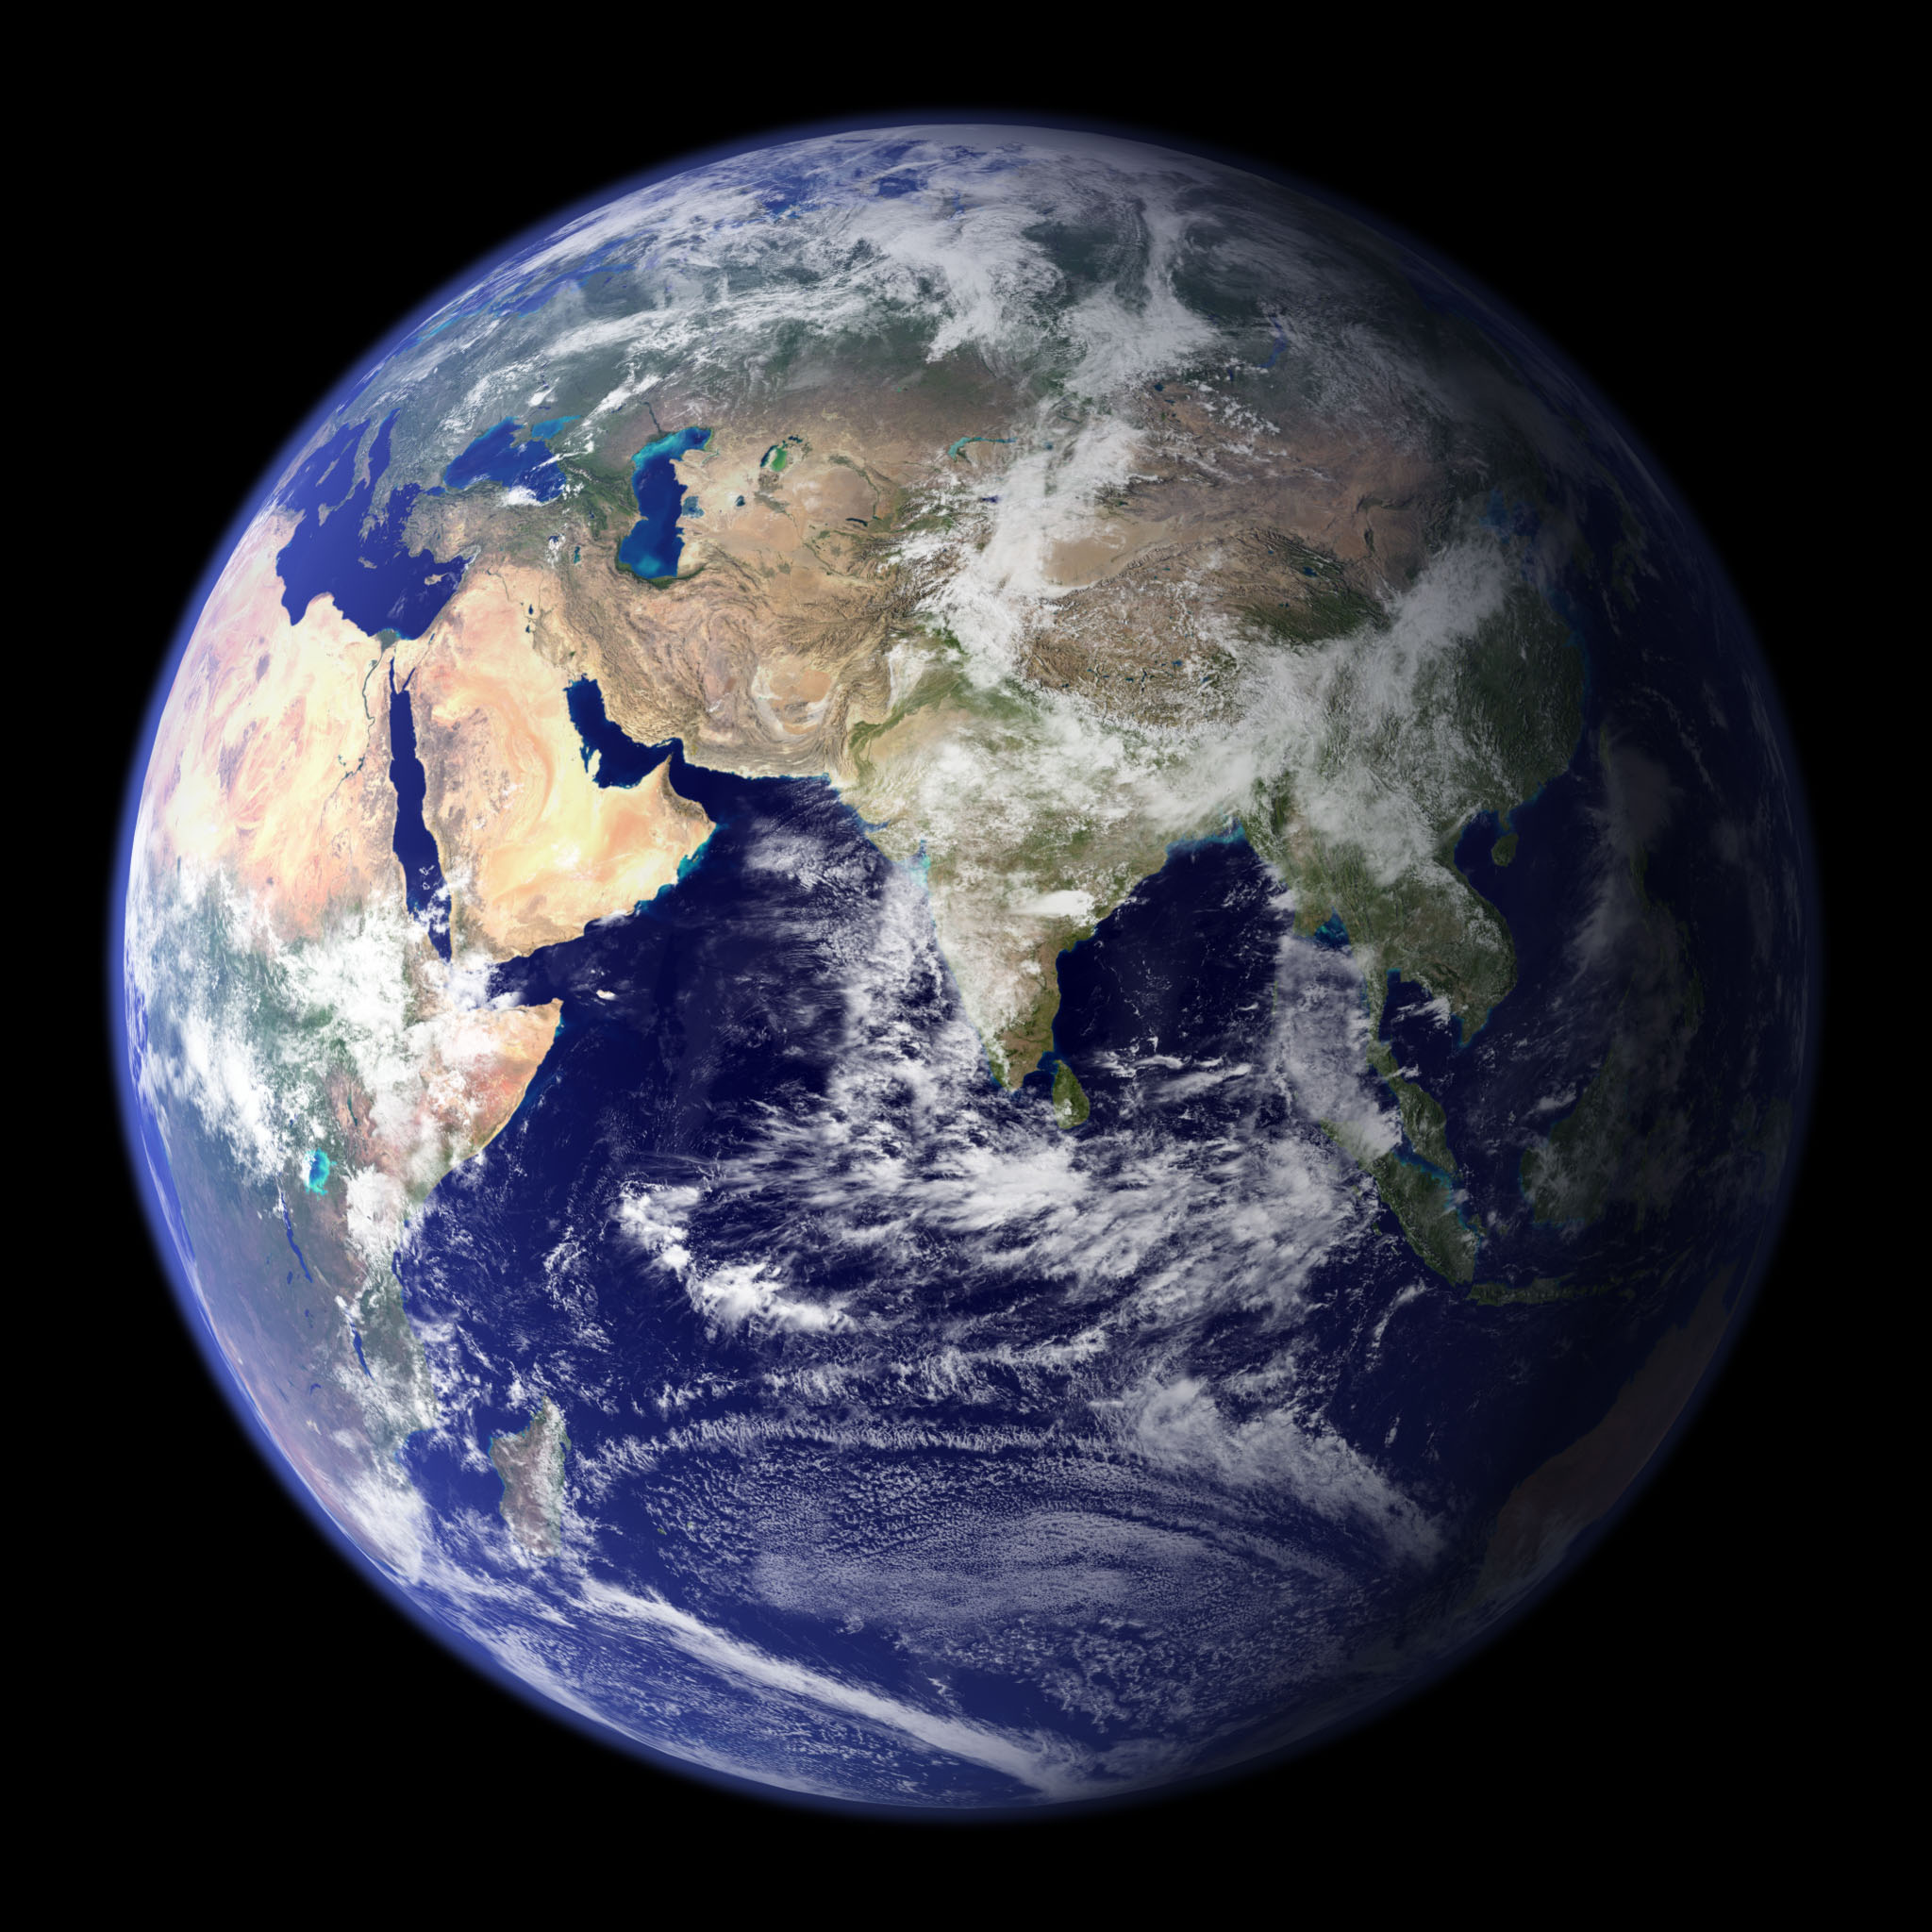
\includegraphics[width=\textwidth]{../images/earth-image.jpg}
            \end{center}
        \end{figure}
    \end{columns}
\end{frame}
}

{
\usebackgroundtemplate{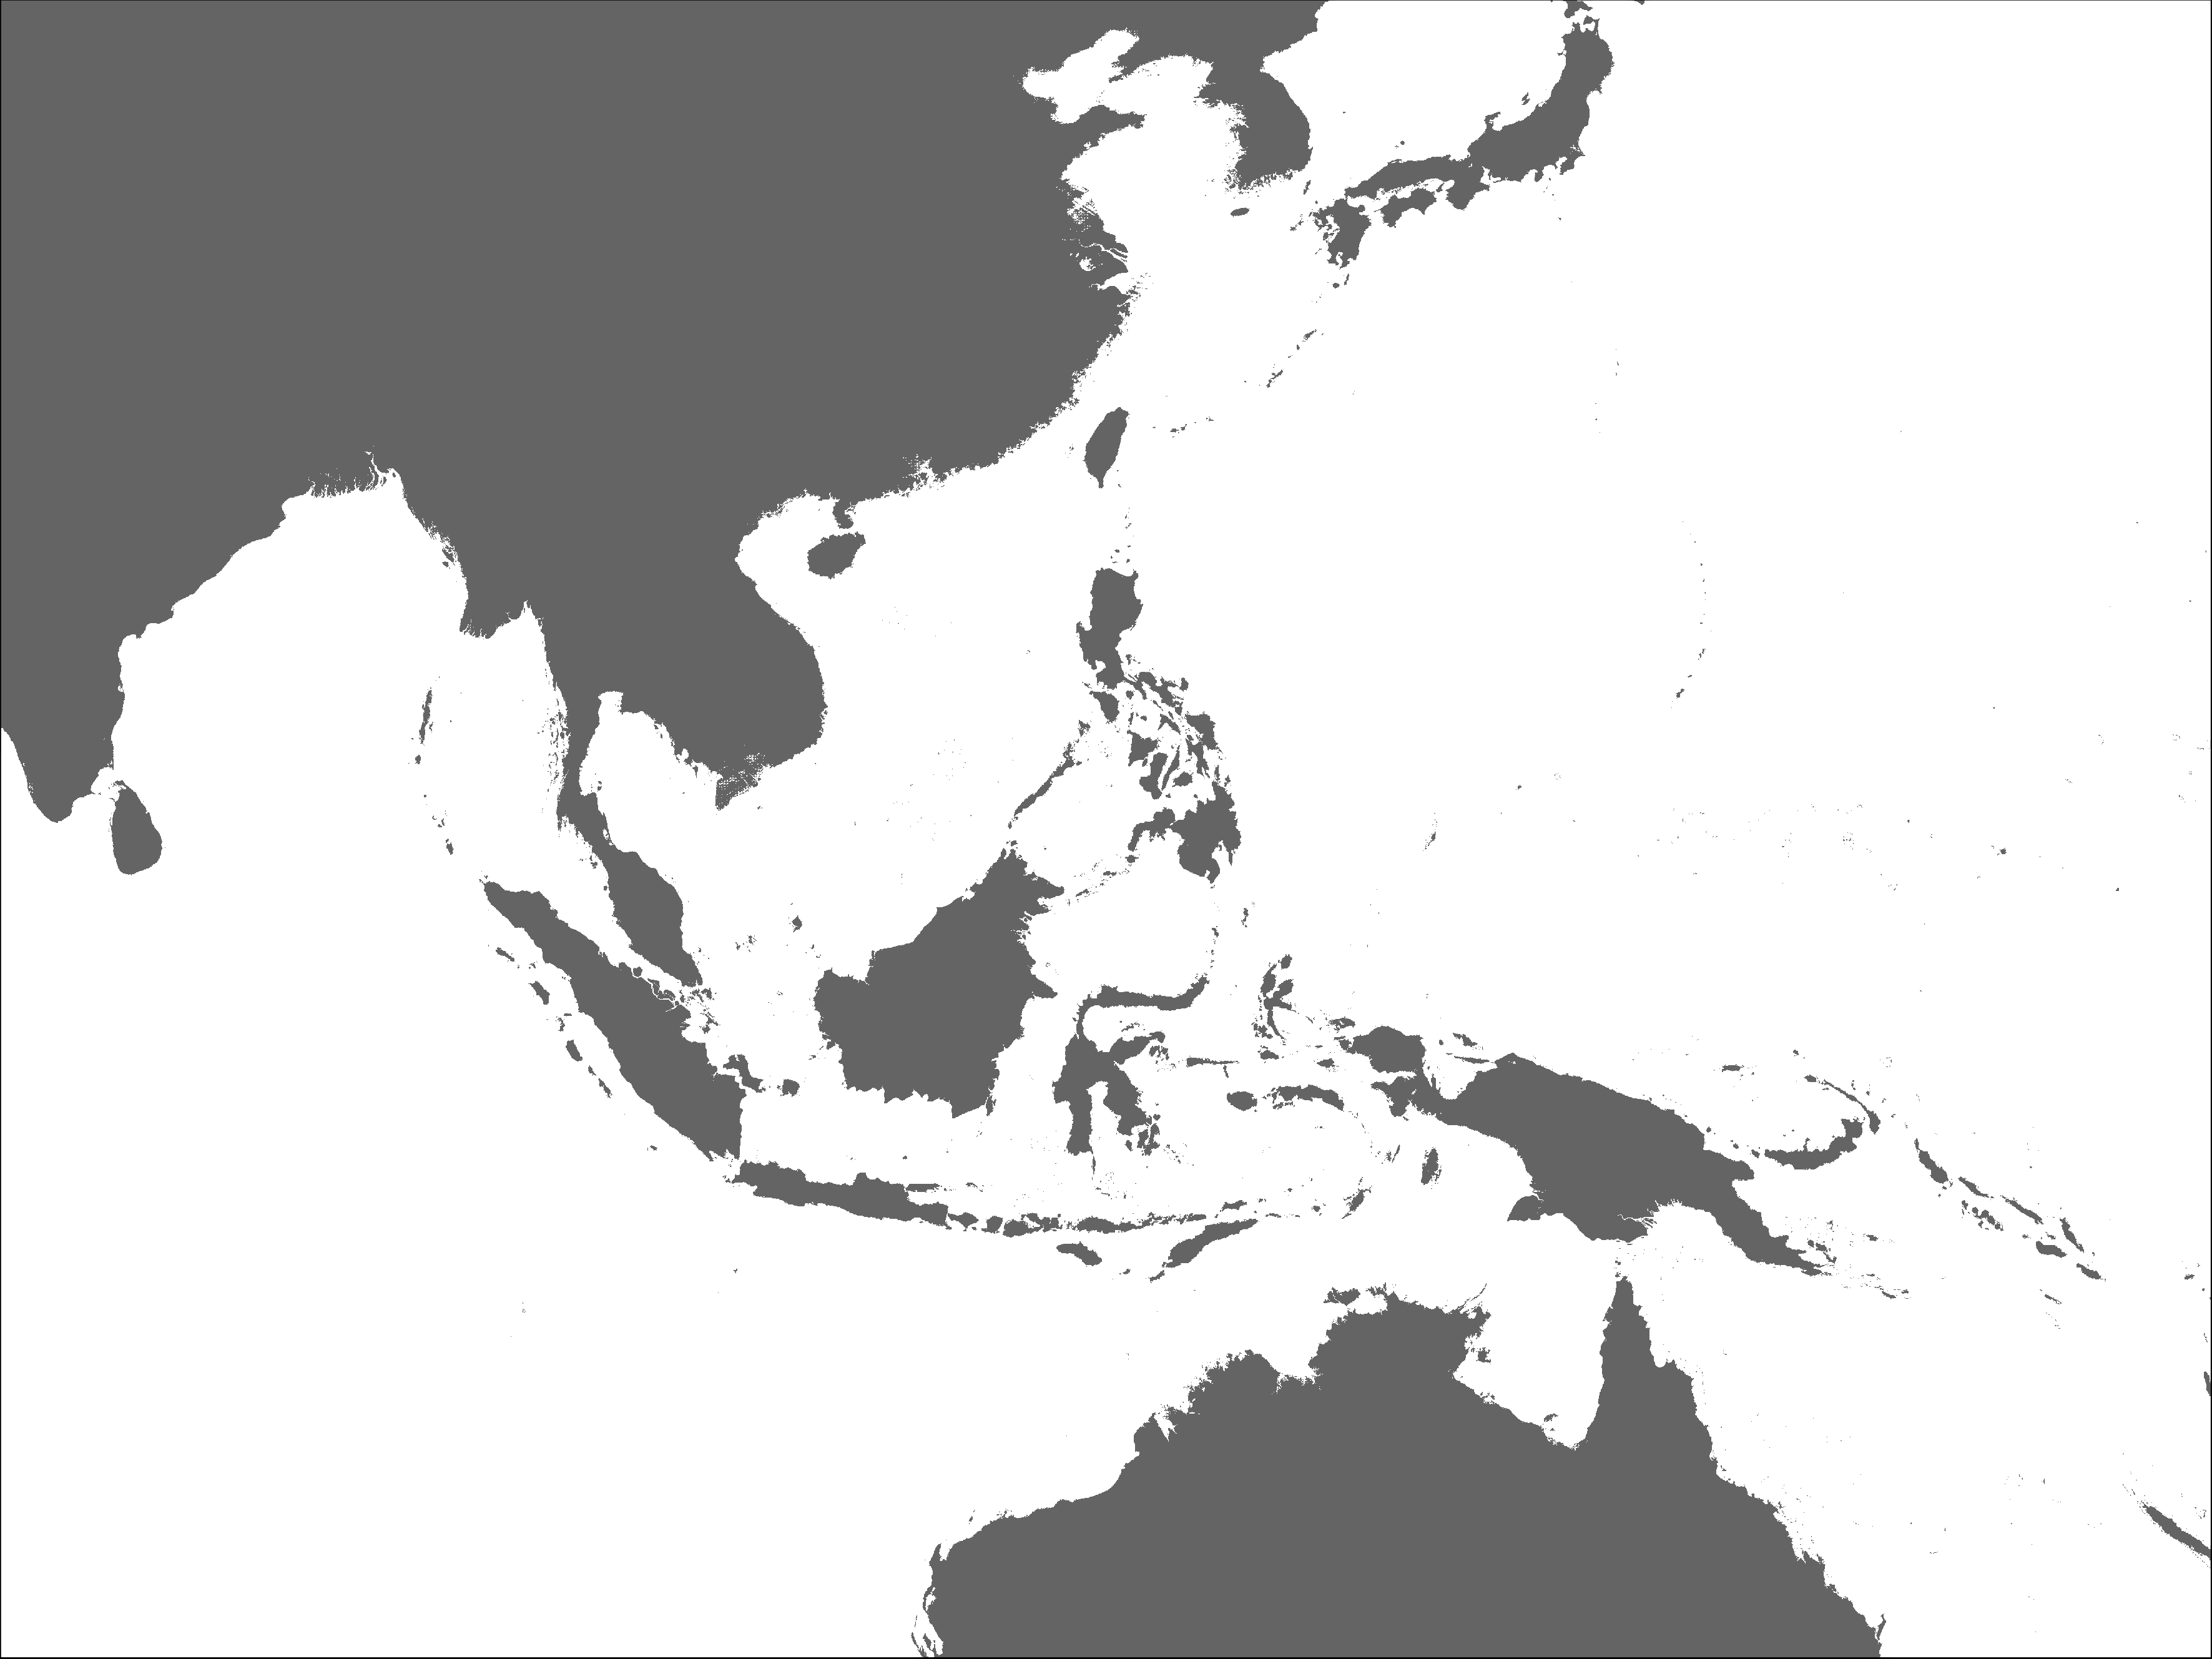
\includegraphics[width=\paperwidth]{../images/maps/se-asia-present.png}}
\begin{frame}
    % \frametitle{Climate-driven diversification}    

\end{frame}
}

{
\usebackgroundtemplate{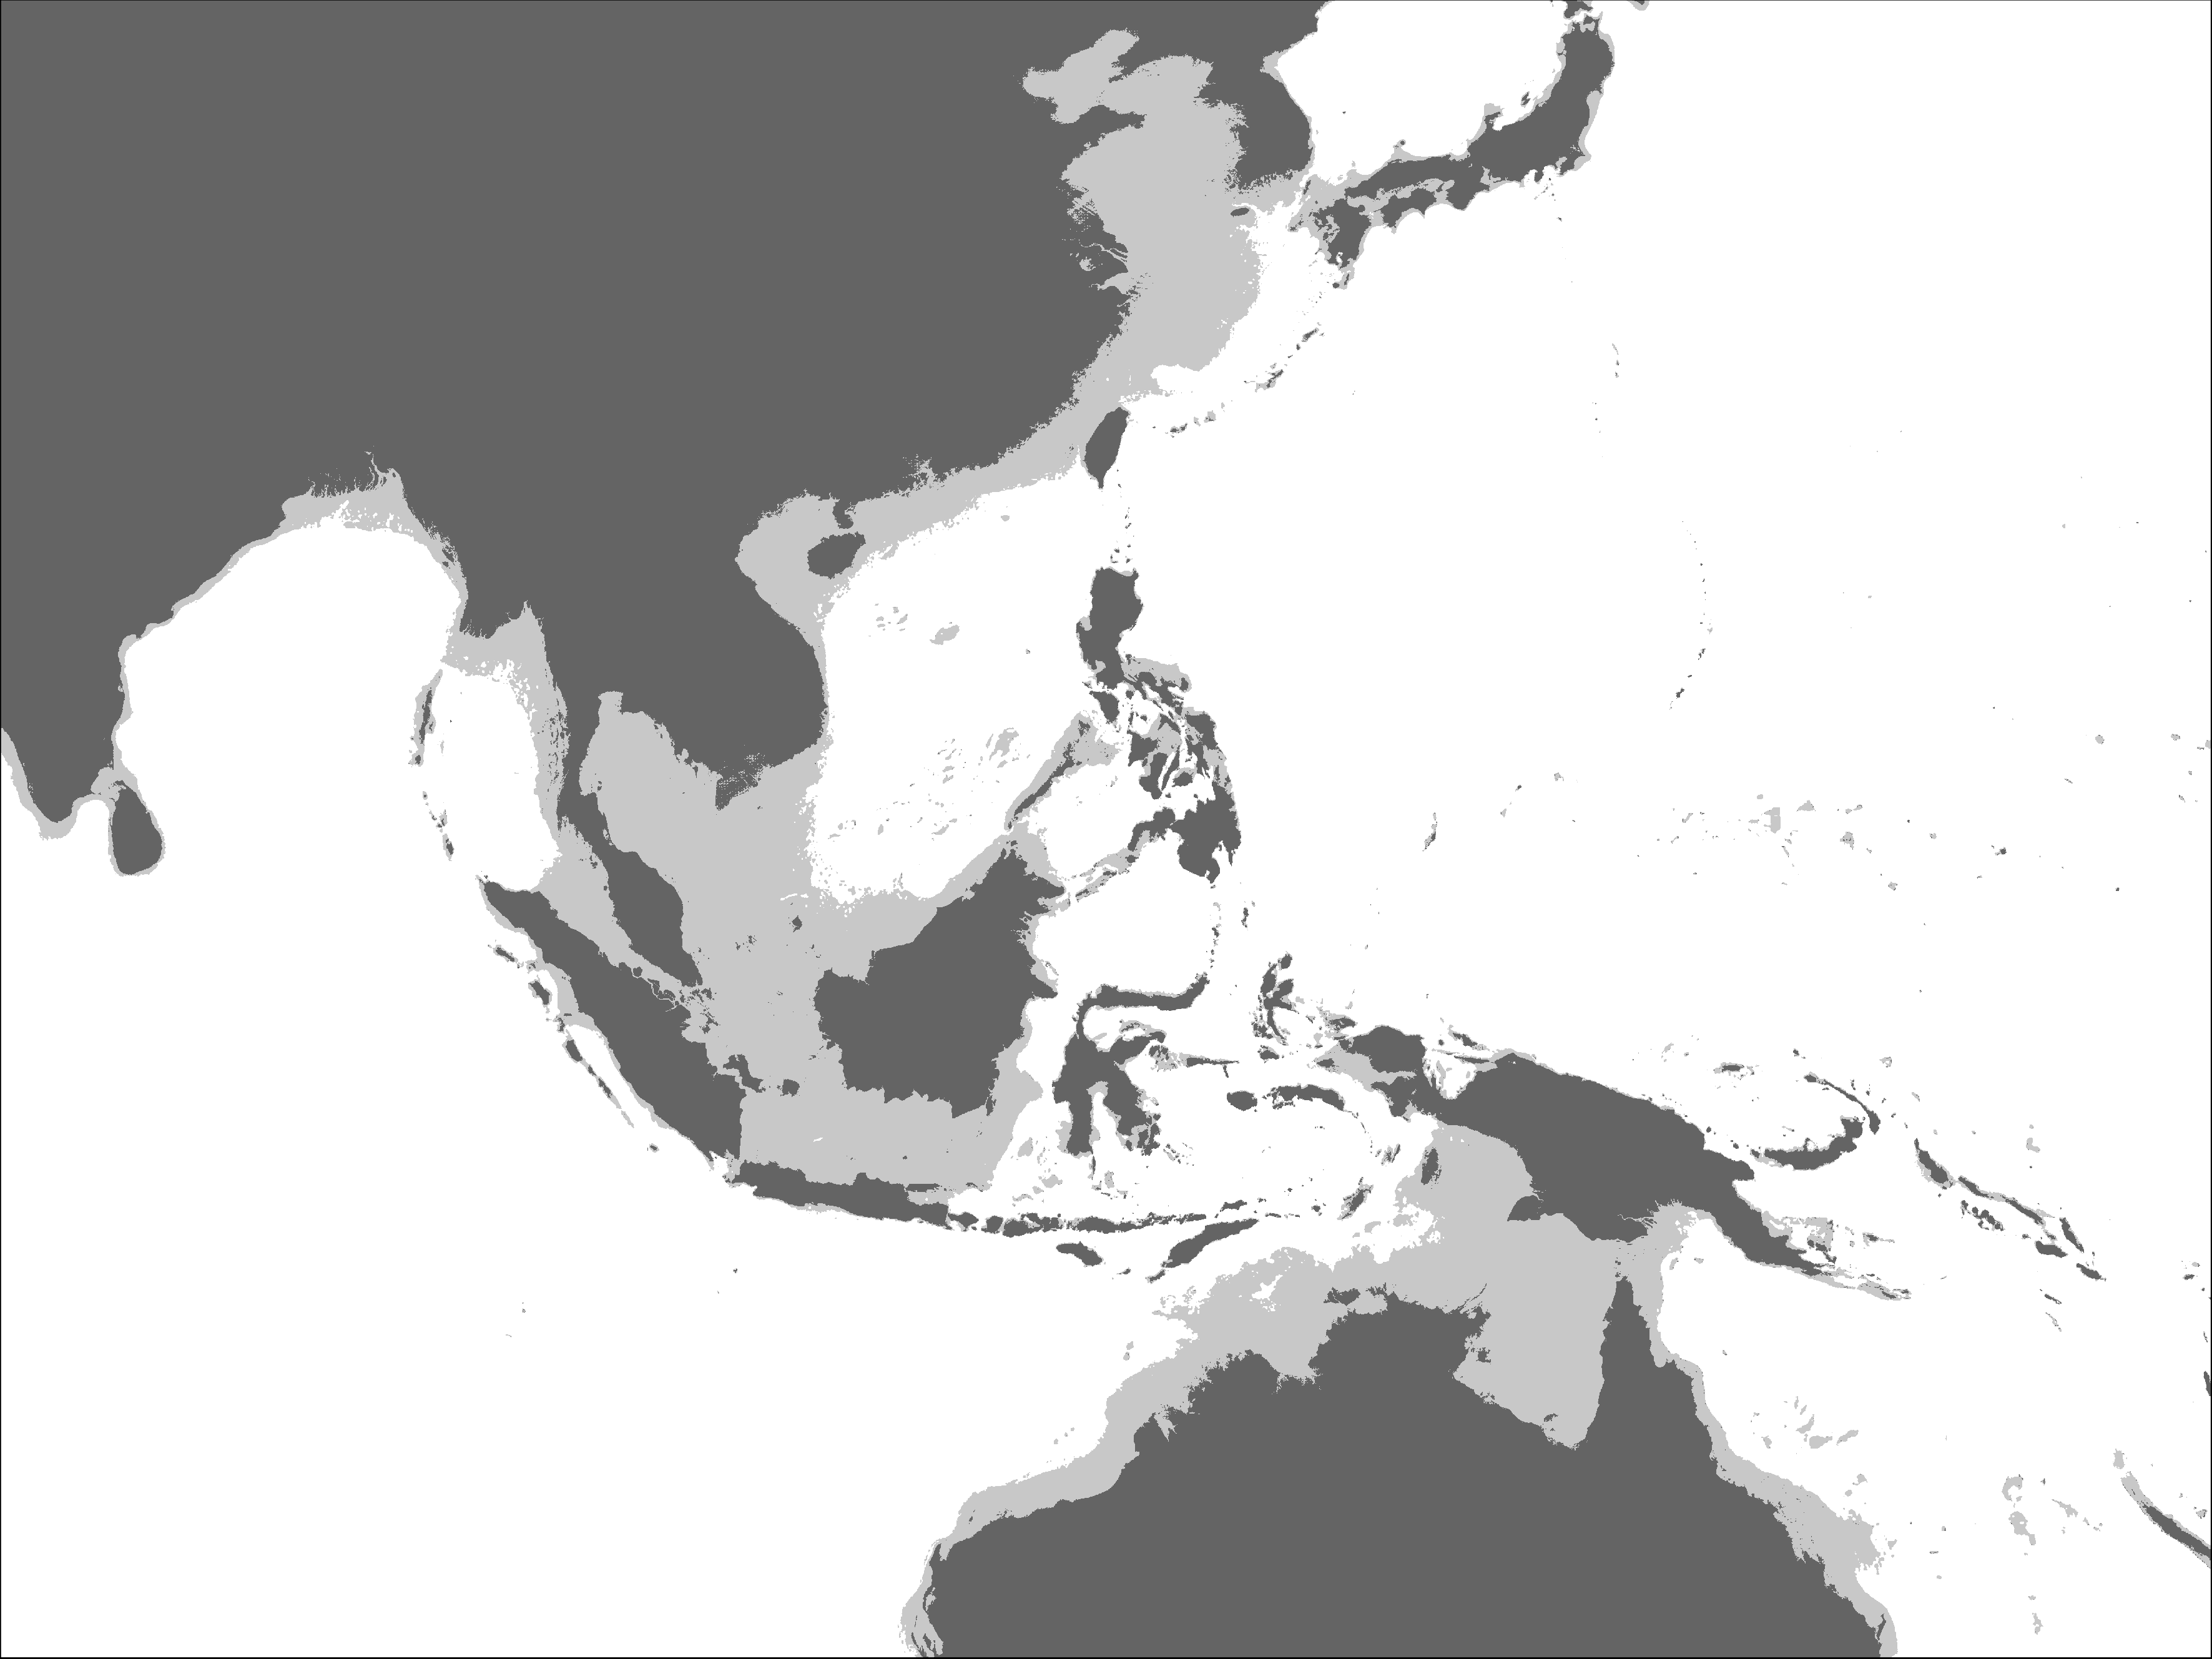
\includegraphics[width=\paperwidth]{../images/maps/se-asia-120.png}}
\begin{frame}
    % \frametitle{Climate-driven diversification}    
    \begin{columns}
        \column{0.6\textwidth}

        \vspace{6.5cm}

        \ \\

        \column{0.4\textwidth}

        \vspace{-2cm}

        \begin{uncoverenv}<2->
        \colorbox{white}{
            \begin{minipage}[t]{1.0\textwidth}
                \raggedright
                \textbf{Did repeated fragmentation of islands during
                    inter-glacial rises in sea level promote diversification?}
            \end{minipage}
        }
        \end{uncoverenv}
    \end{columns}
\end{frame}
}

\begin{frame}
    \frametitle{Climate-driven diversification}
\begin{columns}[c]
    \column{.5\textwidth}
        \vspace{-1cm}
        \begin{onlyenv}<1>
        \begin{minipage}[t][1.0\textheight][c]{\linewidth}
        \centerline{
        \includegraphics<1>[height=2cm]{/home/jamie/Dropbox/field-photos/people/rafe.jpg}
        \hspace{0.3mm}
        \includegraphics<1>[height=2cm]{/home/jamie/Dropbox/field-photos/people/rob.jpg}}
        \centerline{
        \includegraphics<1>[height=2cm]{/home/jamie/Dropbox/field-photos/people/charles.jpg}
        \hspace{0.3mm}
        \includegraphics<1>[height=2cm]{/home/jamie/Dropbox/field-photos/people/cam.jpg}}
        \centerline{
        \includegraphics<1>[height=2cm]{/home/jamie/Dropbox/field-photos/people/jeet2.jpg}
        \hspace{0.3mm}
        \includegraphics<1>[height=2cm]{/home/jamie/Dropbox/field-photos/people/jake.jpg}}
        \centerline{
        \includegraphics<1>[height=2cm]{/home/jamie/Dropbox/field-photos/people/allie.jpg}
        \hspace{0.3mm}
        \includegraphics<1>[height=2cm]{/home/jamie/Dropbox/field-photos/people/Luke.jpg}
        \hspace{0.3mm}
        \includegraphics<1>[height=2cm]{/home/jamie/Dropbox/field-photos/people/anthony.png}}
        \end{minipage}
        \end{onlyenv}

        \begin{onlyenv}<2->
        \begin{minipage}[t][1.0\textheight][c]{\linewidth}
        \centerline{
        \includegraphics<2->[height=1.3cm]{../images/photos/crocidura-negrina-JAEsselstyn.jpg}
        \hspace{0.3mm}
        \includegraphics<2->[height=1.3cm]{../images/photos/crocidura-beatus-DSBalete.jpg}}
        % \vspace{0.5mm}
        \centerline{
        \includegraphics<2->[height=1.3cm]{../images/photos/hipposideros-obscurus-MRMDuya.jpg}
        \hspace{0.3mm}
        \includegraphics<2->[height=1.3cm]{../images/photos/haplonycteris-fischeri-JHolden.jpg}}
        % \vspace{0.5mm}
        \centerline{
        \includegraphics<2->[height=1.3cm]{../images/photos/sphenomorphus-abdictus-rmb.jpg}
        \hspace{0.3mm}
        \includegraphics<2->[height=1.3cm]{../images/photos/sphenomorphus-arborens-rmb.jpg}}
        % \vspace{0.5mm}
        \centerline{
        \includegraphics<2->[height=1.3cm]{../images/photos/gekko-mindorensis.jpg}
        \hspace{0.3mm}
        \includegraphics<2->[height=1.3cm]{../images/photos/dendrelaphis-pictus-cds.jpg}}
        % \vspace{0.5mm}
        \centerline{
        \includegraphics<2->[height=1.3cm]{../images/photos/cyrt-agusanensis.jpg}
        \hspace{0.3mm}
        \includegraphics<2->[height=1.3cm]{../images/photos/cyrt-annulatus-cds.jpg}}
        % \vspace{0.5mm}
        \centerline{
        \includegraphics<2->[height=1.3cm]{../images/photos/limnonectes-magnus-cds.jpg}
        \hspace{0.3mm}
        \includegraphics<2->[height=1.3cm]{../images/photos/limnonectes-leytensis-rmb.jpg}}
        \end{minipage}
        \end{onlyenv}

    \column{.5\textwidth}
        \vspace{-1cm}
        \begin{minipage}[t][1.0\textheight][c]{\linewidth}
        \includegraphics<1-2>[width=\textwidth]{../images/maps/Philippines.png}
        \includegraphics<3>[width=\textwidth]{../images/maps/Philippines-negros_panay.png}
        % \begin{onlyenv}<4->
        %     \begin{itemize}
        %         \item Strong support for simultaneous divergence of all 22 taxon pairs
                
        %         \item Posterior probability $>$ 0.96 \\
            
        %         \item $\sim$100,000--250,000 years ago
        %     \end{itemize}
        % \end{onlyenv}
        \end{minipage}
\end{columns}
\end{frame}


\begin{frame}[t]
    % \frametitle<1-4>{Climate-driven diversification: Predictions}
    % \frametitle<5->{Divergence-model choice}
    \frametitle{Inferring community history}

    \centering{
    % \includegraphics<1>[height=7.5cm]{../images/dmc-cartoon-islands.pdf}
    % \includegraphics<2>[height=7.5cm]{../images/dmc-cartoon-taxa.pdf}
    \includegraphics<1>[height=7.5cm]{../images/dmc-cartoon-sea-level.pdf}
    % \includegraphics<4>[height=7.5cm]{../images/dmc-cartoon-shared-no-labels.pdf}
    \includegraphics<2>[height=7.5cm]{../images/dmc-cartoon-shared.pdf}
    \includegraphics<3>[height=7.5cm]{../images/dmc-cartoon-2-1.pdf}
    \includegraphics<4>[height=7.5cm]{../images/dmc-cartoon-2-2.pdf}
    \includegraphics<5>[height=7.5cm]{../images/dmc-cartoon-2-3.pdf}
    \includegraphics<6>[height=7.5cm]{../images/dmc-cartoon-general.pdf}
    }
\end{frame}


\begin{frame}[t]
    % \frametitle{Divergence-model choice}
    \frametitle{Inferring community history}

    \vspace{-7mm}

    \begin{minipage}[t][0.1\textheight][c]{1.1\linewidth}
        \begin{adjustwidth}{-0.5em}{}
            \begin{tabular}{ p{2.1cm} p{2.1cm} p{2.1cm} p{2.1cm} p{2.1cm} }
                $m_1$ & $m_2$ & $m_3$ & $m_4$ & $m_5$ \\
            \end{tabular}
        \end{adjustwidth}
    \end{minipage}

    \vspace{-2mm}

    \begin{minipage}[t][0.35\textheight][c]{1.1\linewidth}
        \begin{adjustwidth}{-2.3em}{}
        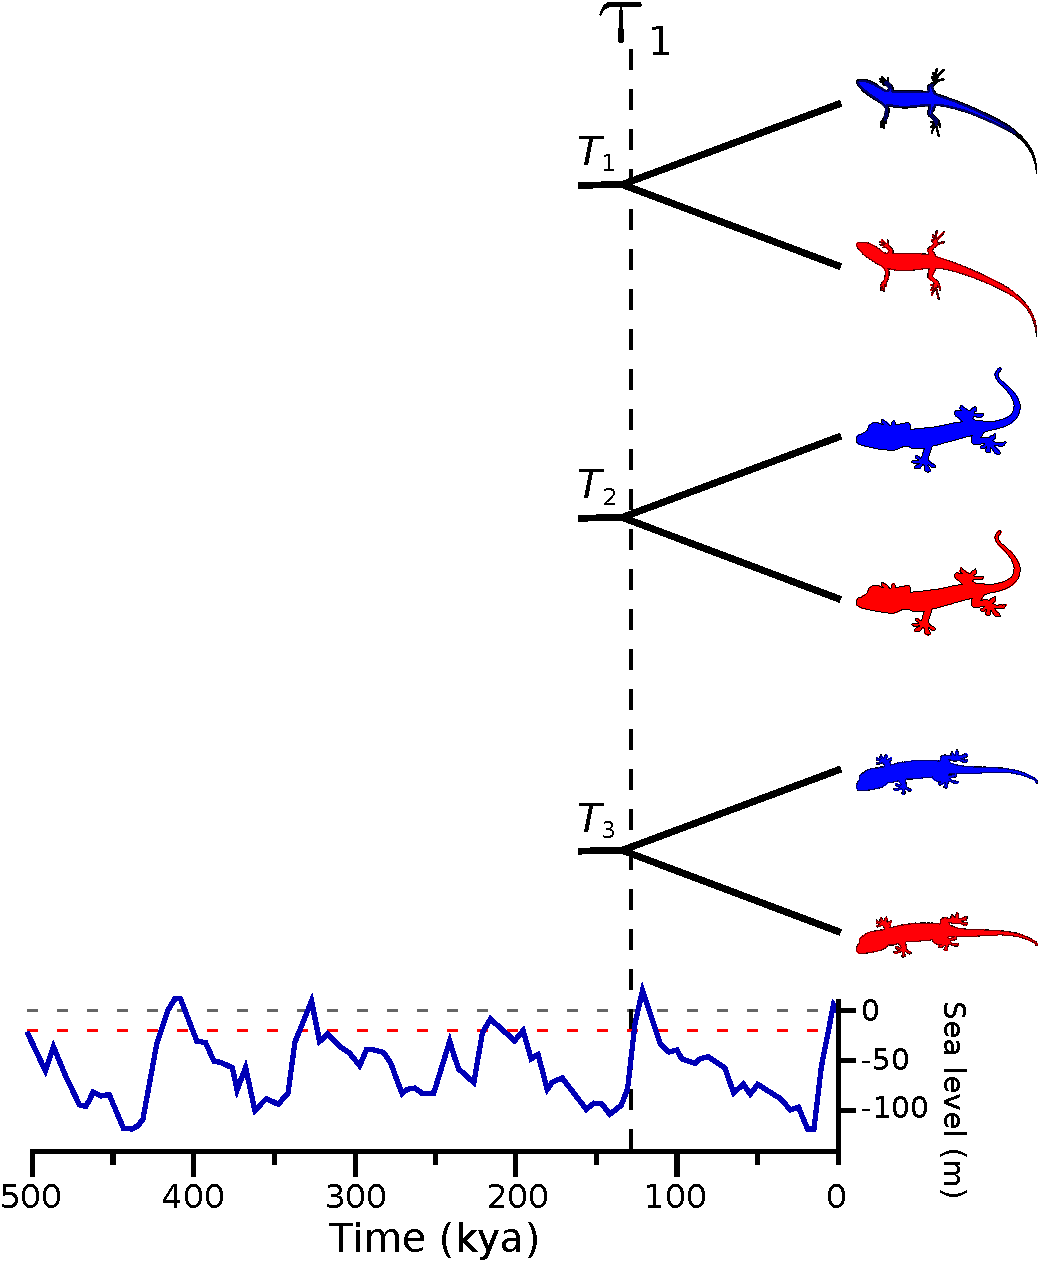
\includegraphics[height=2.9cm]{../images/dmc-cartoon-no-islands-shared.pdf}
        \hspace{0.2mm}
        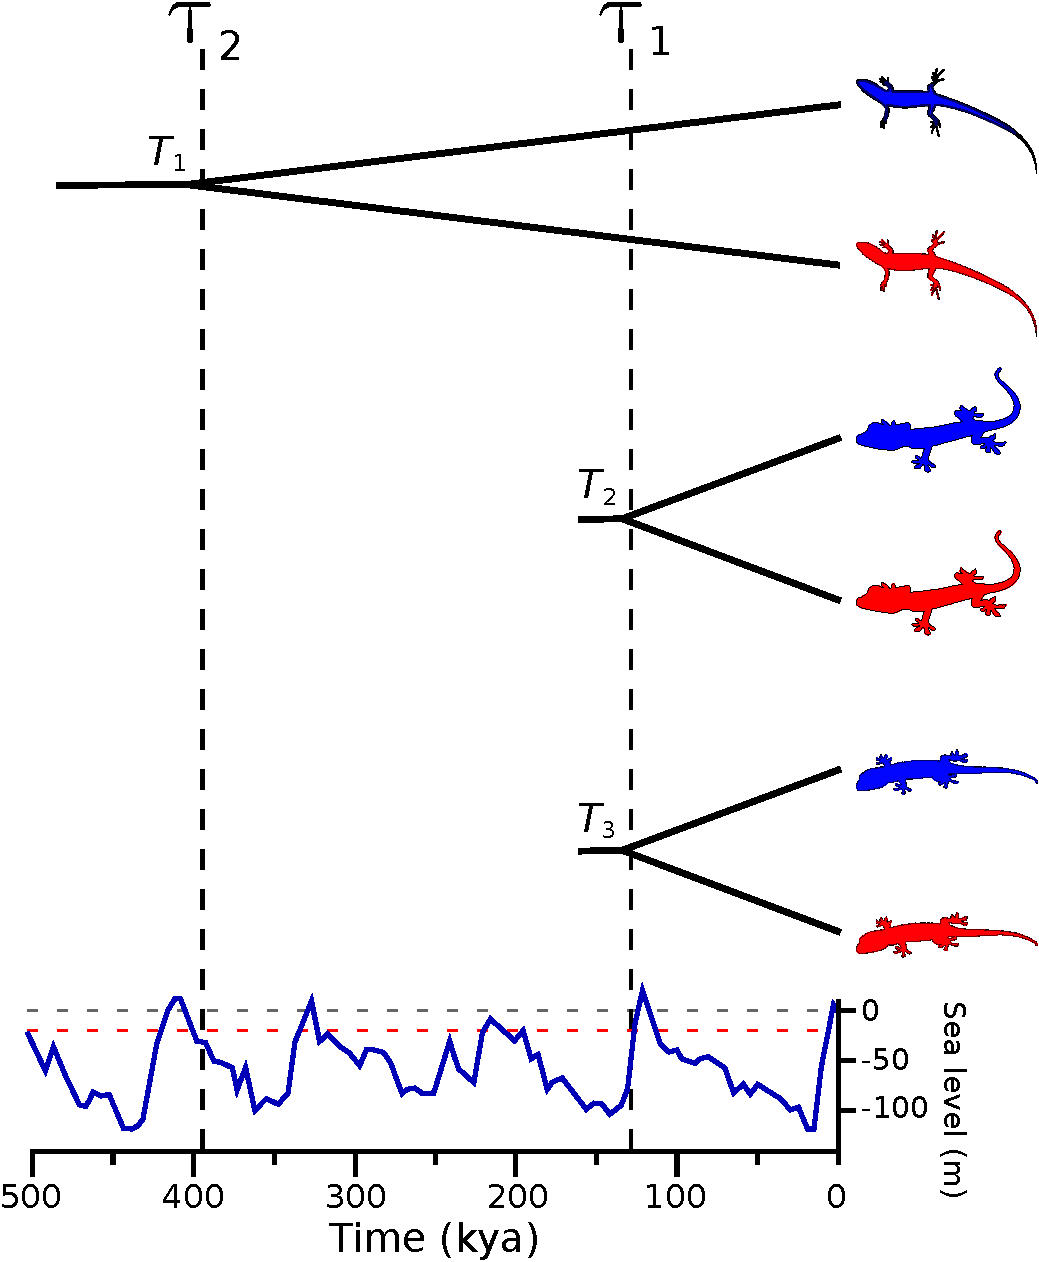
\includegraphics[height=2.9cm]{../images/dmc-cartoon-no-islands-2-1.pdf}
        \hspace{0.2mm}
        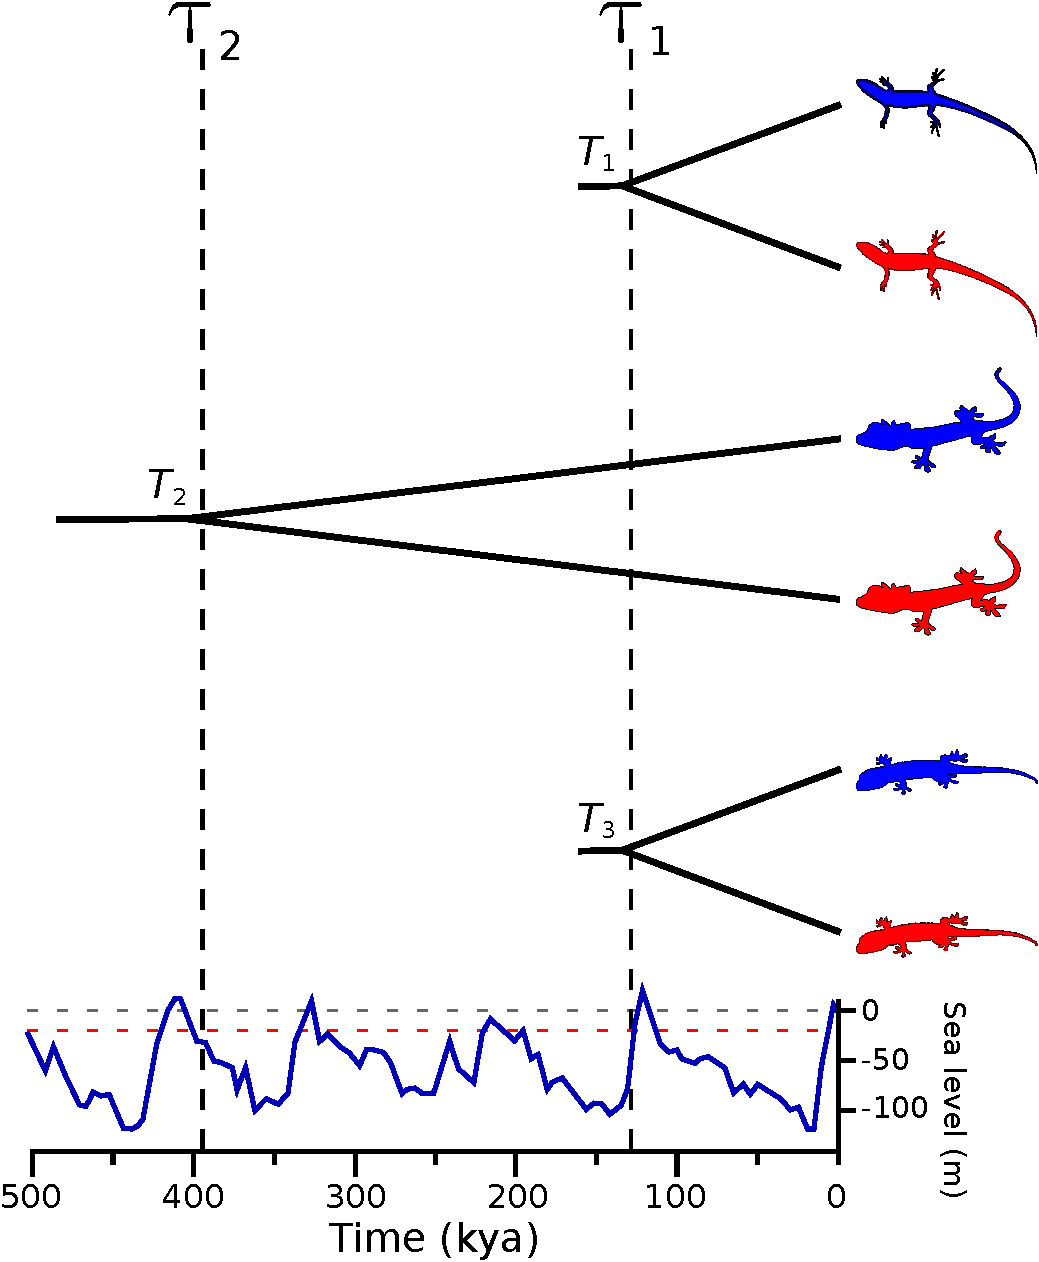
\includegraphics[height=2.9cm]{../images/dmc-cartoon-no-islands-2-2.pdf}
        \hspace{0.2mm}
        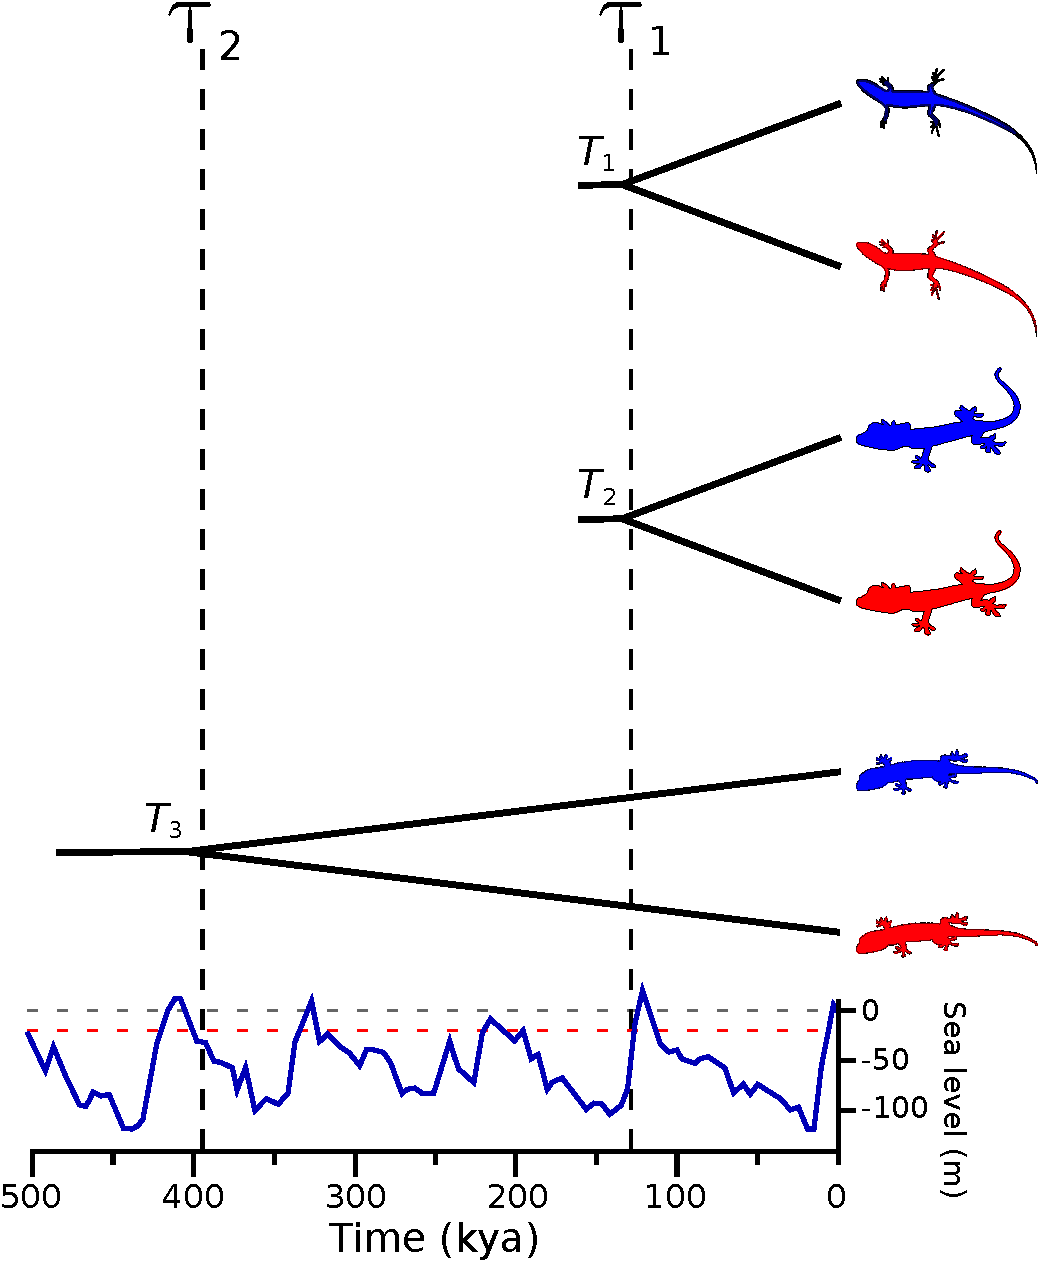
\includegraphics[height=2.9cm]{../images/dmc-cartoon-no-islands-2-3.pdf}
        \hspace{0.2mm}
        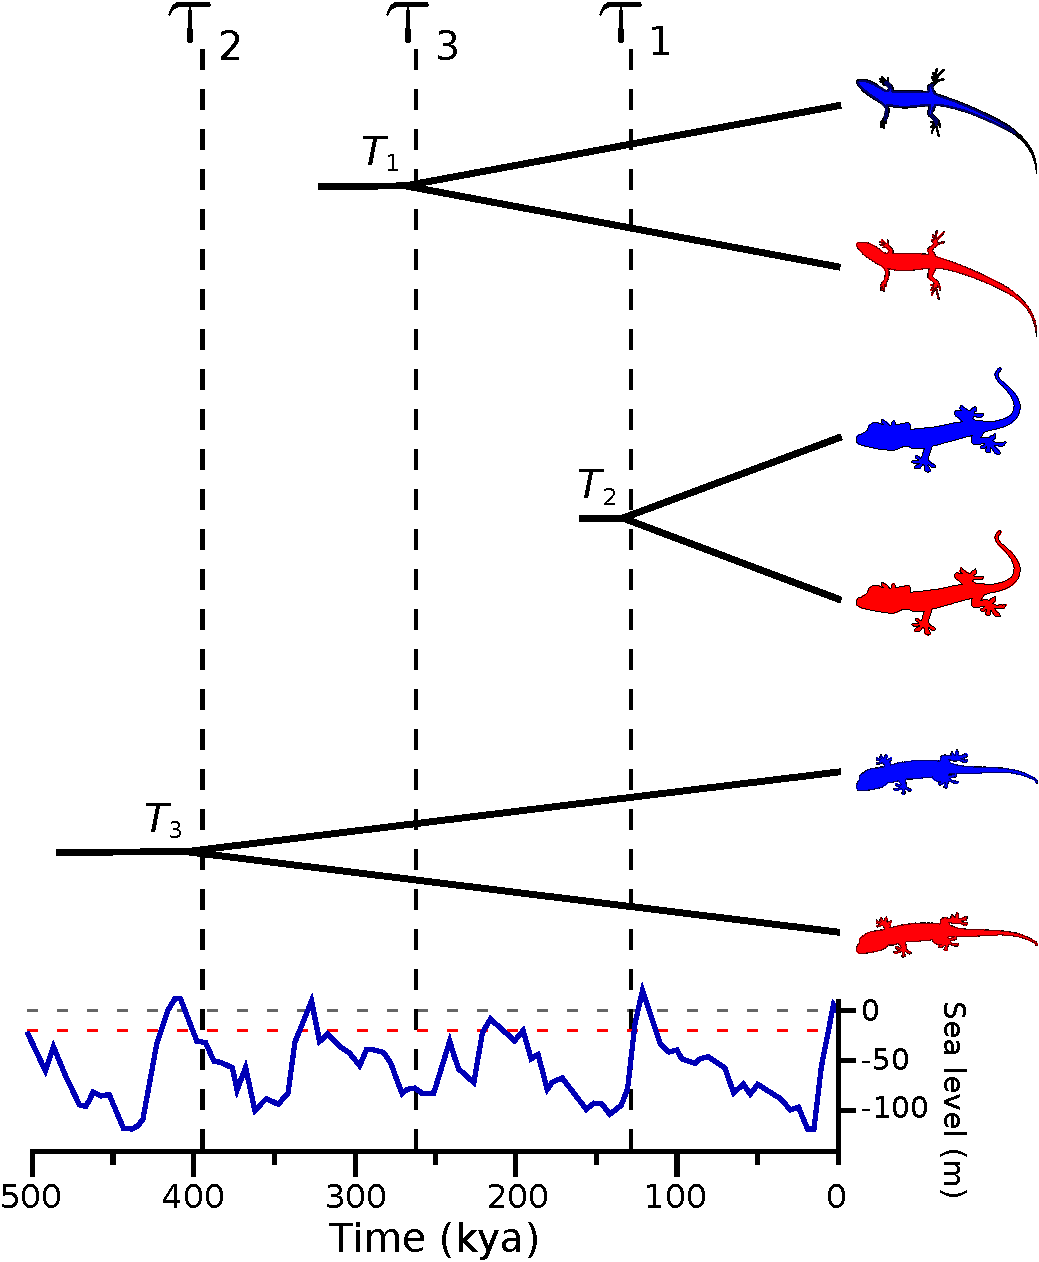
\includegraphics[height=2.9cm]{../images/dmc-cartoon-no-islands-general.pdf}
        \end{adjustwidth}
    \end{minipage}

    \vspace{3.5mm}

    \begin{minipage}[c][0.35\textheight][c]{\linewidth}
        \begin{uncoverenv}<2->
            \begin{center}
            We want to infer \textcolor{blue}{\divModel{}} and
            \textcolor{blue}{\divTimeMapVector} given DNA sequence
            alignments
            \textcolor{blue}{\alignmentVector}
        \end{center}
        \end{uncoverenv}

        \vspace{4mm}

        \begin{uncoverenv}<3->
            \begin{displaybox}[0.85\linewidth]
                \begin{minipage}[c][0.12\textheight][c]{\linewidth}

                \[
                    p(\divTimeMapVector,
                      \divModel{i},
                      \allParameters{}
                      \given \alignmentVector)
                      =
                    \frac{
                        p(\alignmentVector \given
                          \divTimeMapVector,
                          \allParameters{},
                          \divModel{i})
                        p(\divTimeMapVector,
                          \allParameters{}
                          \given \divModel{i})
                        p(\divModel{i})
                        }{p(\alignmentVector)}
                \]
                \vspace{-1mm}
                \end{minipage}
            \end{displaybox}
        \end{uncoverenv}
    \end{minipage}
\end{frame}

\begin{frame}
    \frametitle{New method: \dppmsbayes}
    \begin{itemize}
        % \item<1-> Reparameterized the model implemented in \msb
        \item<1-> Dirichlet-process prior (DPP) over all possible divergence
            models
        \item<2-> Flexible priors on continuous parameters to avoid strongly
            weighted posteriors
        \item<3-> Multi-processing interface to accommodate genomic datasets
        % \item<4-> Uniform prior over divergence models
    \end{itemize}
    \barefootnote{\shortfullcite{Oaks2014dpp}}
\end{frame}

\begin{frame}
    \frametitle{\dppmsbayes: Performance}
    \begin{itemize}
        \item<1-> Extensive computer simulations to compare performance to previous
            state-of-the-art methods (\msb).
        \item<2-> New method for estimating shared evolutionary history shows
            improved:
            \begin{enumerate}
                \item<2-> Improved model-choice accuracy 
                \item<2-> More robustness to model violations
                \item<2-> Greater power to detect variation in divergence times
                \item<2-> Faster!
            \end{enumerate}
    \end{itemize}

    \uncover<3->{
    \textbf{\dppmsbayes allows biologists to leverage comparative genomic data
        to assess the affects of community-scale processes on biodiversity}
    }
    \barefootnote{\shortfullcite{Oaks2014dpp}}
\end{frame}

{
\usebackgroundtemplate{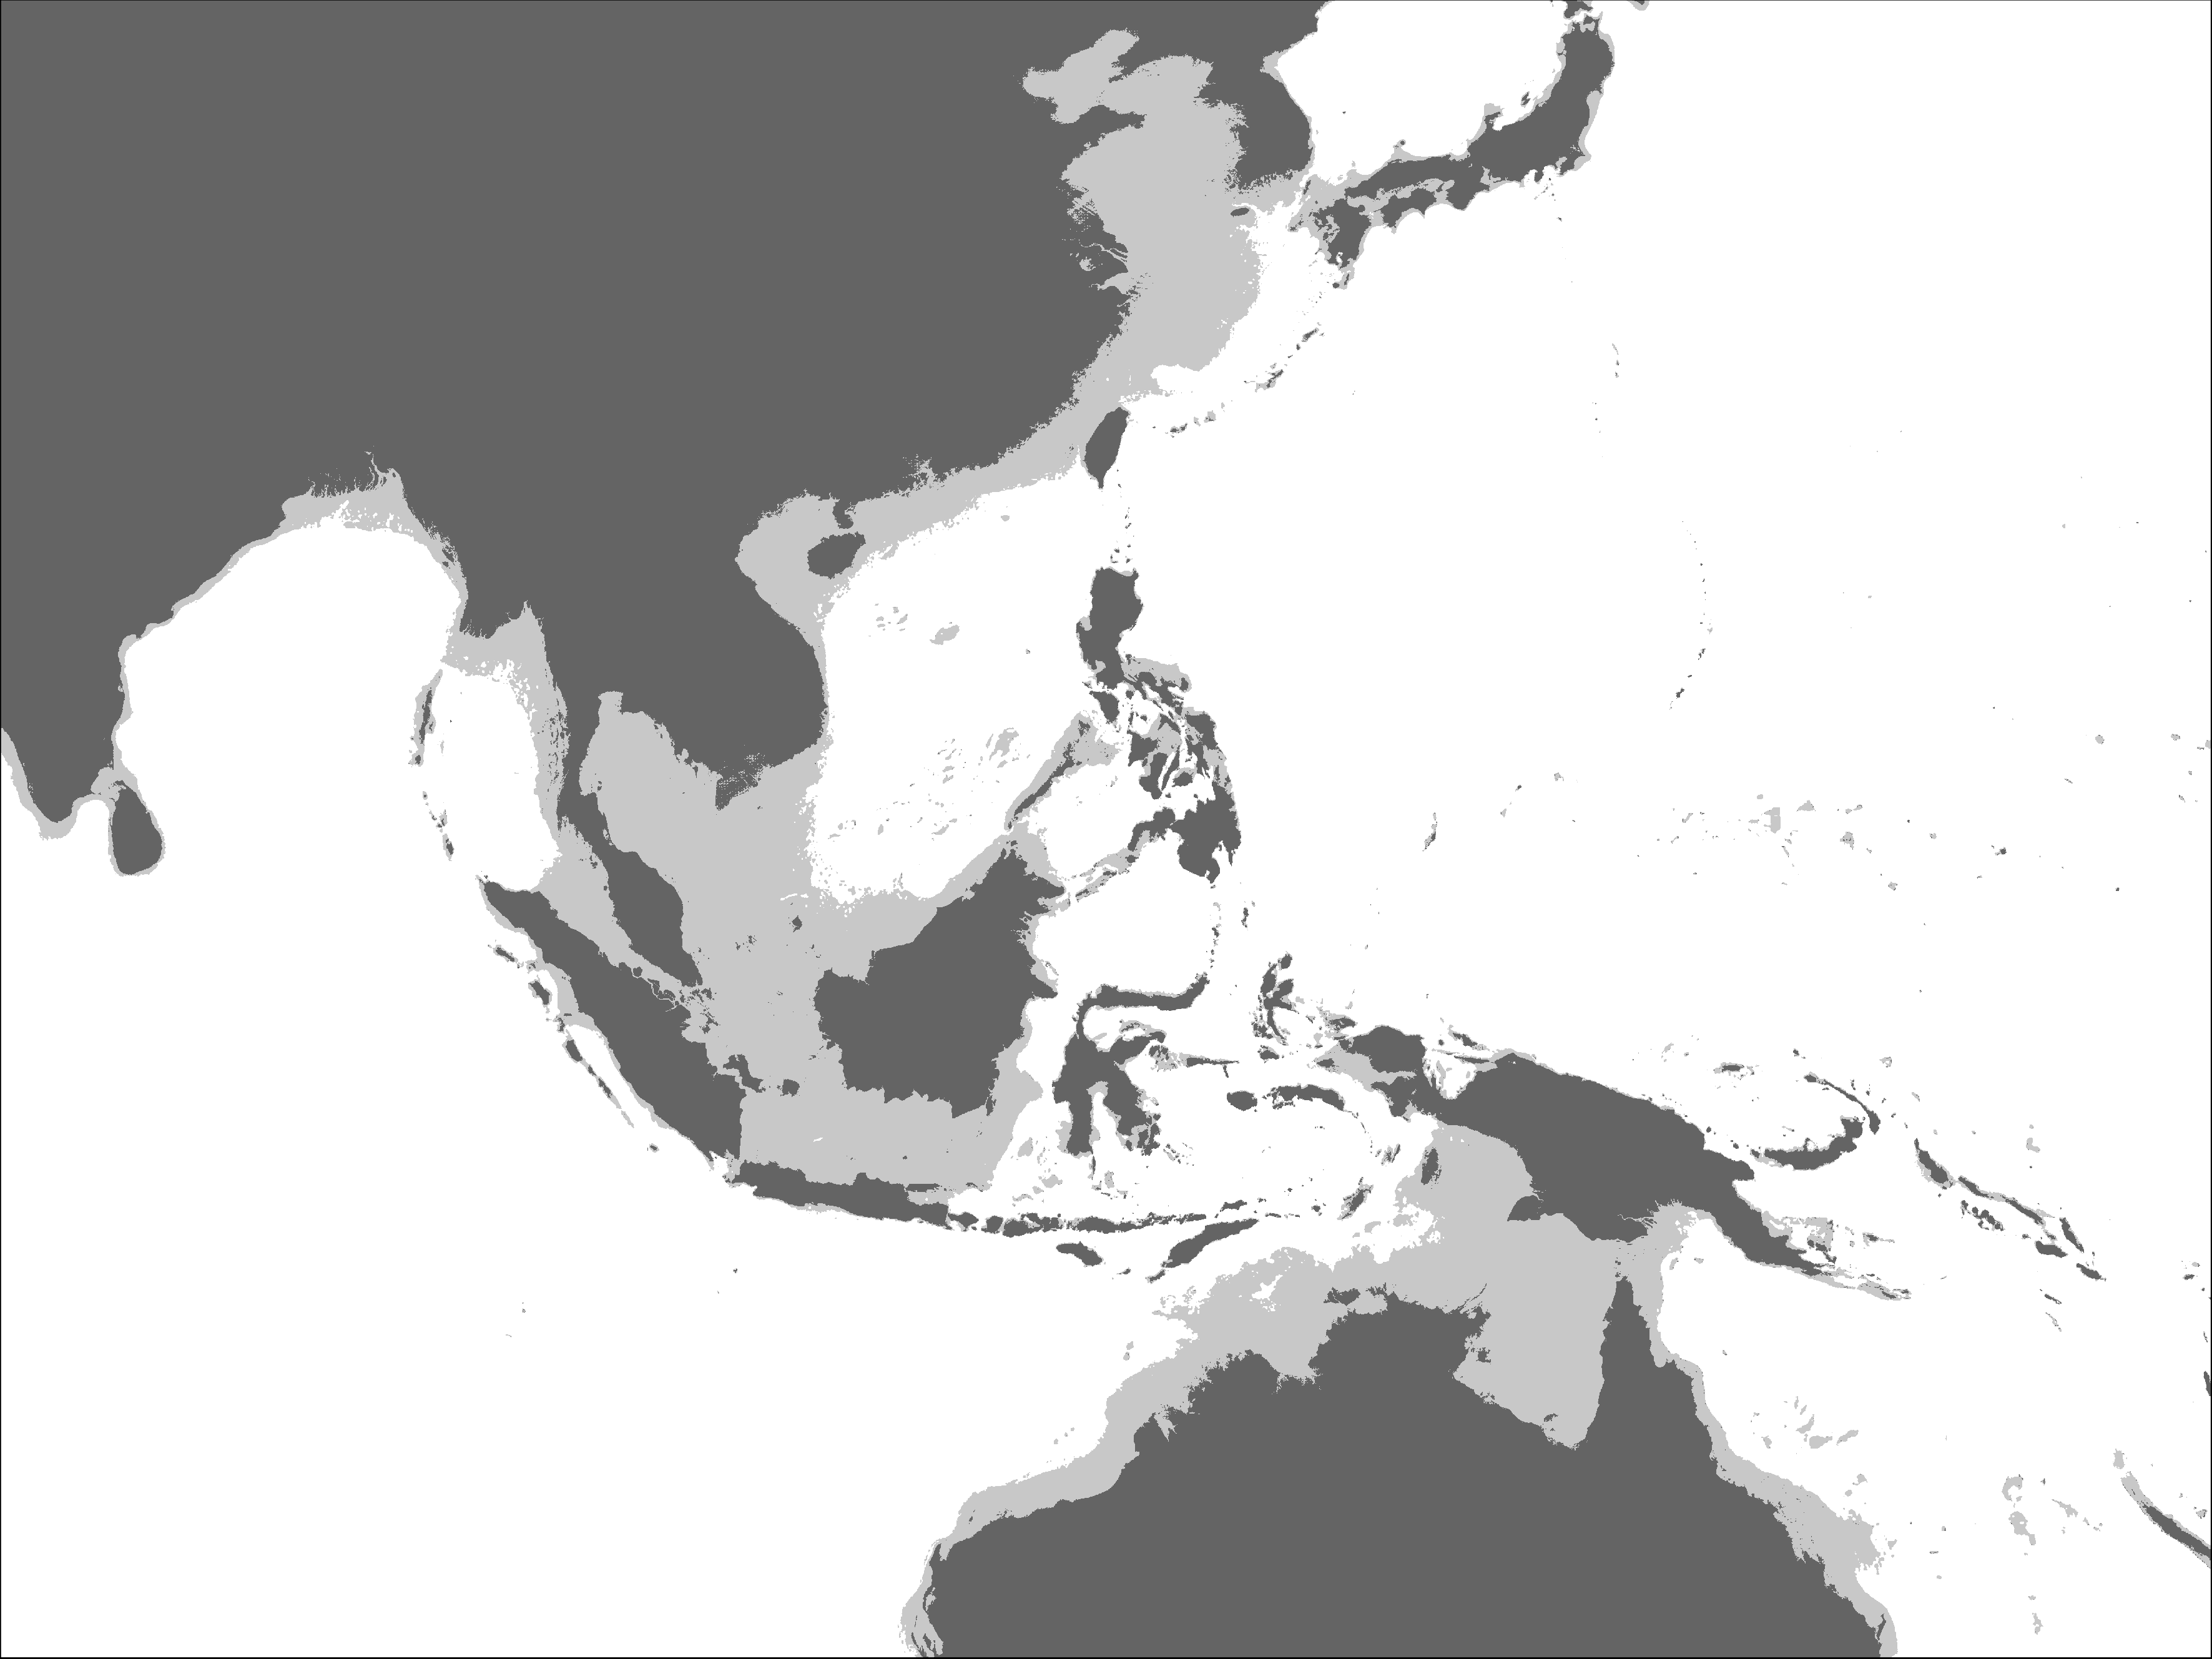
\includegraphics[width=\paperwidth]{../images/maps/se-asia-120.png}}
\begin{frame}
    % \frametitle{Climate-driven diversification}    
    \begin{columns}
        \column{0.6\textwidth}

        \vspace{6.5cm}

        \ \\

        \column{0.4\textwidth}

        \vspace{-2cm}

        \begin{uncoverenv}<1->
        \colorbox{white}{
            \begin{minipage}[t]{1.0\textwidth}
                \raggedright
                \textbf{Did repeated fragmentation of islands during
                    inter-glacial rises in sea level promote diversification?}
            \end{minipage}
        }
        \end{uncoverenv}
    \end{columns}
\end{frame}
}

\begin{frame}
    \frametitle{Climate-driven diversification}
\begin{columns}[c]
    \column{.5\textwidth}
        \vspace{-1cm}
        \begin{onlyenv}<1->
        \begin{minipage}[t][1.0\textheight][c]{\linewidth}
        \centerline{
        \includegraphics<1->[height=1.3cm]{../images/photos/crocidura-negrina-JAEsselstyn.jpg}
        \hspace{0.3mm}
        \includegraphics<1->[height=1.3cm]{../images/photos/crocidura-beatus-DSBalete.jpg}}
        % \vspace{0.5mm}
        \centerline{
        \includegraphics<1->[height=1.3cm]{../images/photos/hipposideros-obscurus-MRMDuya.jpg}
        \hspace{0.3mm}
        \includegraphics<1->[height=1.3cm]{../images/photos/haplonycteris-fischeri-JHolden.jpg}}
        % \vspace{0.5mm}
        \centerline{
        \includegraphics<1->[height=1.3cm]{../images/photos/sphenomorphus-abdictus-rmb.jpg}
        \hspace{0.3mm}
        \includegraphics<1->[height=1.3cm]{../images/photos/sphenomorphus-arborens-rmb.jpg}}
        % \vspace{0.5mm}
        \centerline{
        \includegraphics<1->[height=1.3cm]{../images/photos/gekko-mindorensis.jpg}
        \hspace{0.3mm}
        \includegraphics<1->[height=1.3cm]{../images/photos/dendrelaphis-pictus-cds.jpg}}
        % \vspace{0.5mm}
        \centerline{
        \includegraphics<1->[height=1.3cm]{../images/photos/cyrt-agusanensis.jpg}
        \hspace{0.3mm}
        \includegraphics<1->[height=1.3cm]{../images/photos/cyrt-annulatus-cds.jpg}}
        % \vspace{0.5mm}
        \centerline{
        \includegraphics<1->[height=1.3cm]{../images/photos/limnonectes-magnus-cds.jpg}
        \hspace{0.3mm}
        \includegraphics<1->[height=1.3cm]{../images/photos/limnonectes-leytensis-rmb.jpg}}
        \end{minipage}
        \end{onlyenv}

    \column{.5\textwidth}
        \vspace{-1cm}
        \begin{minipage}[t][1.0\textheight][c]{\linewidth}
        \includegraphics<1->[width=\textwidth]{../images/maps/Philippines.png}
        \end{minipage}
\end{columns}
\end{frame}


\begin{frame}
    \frametitle{Results}
    \centerline{
    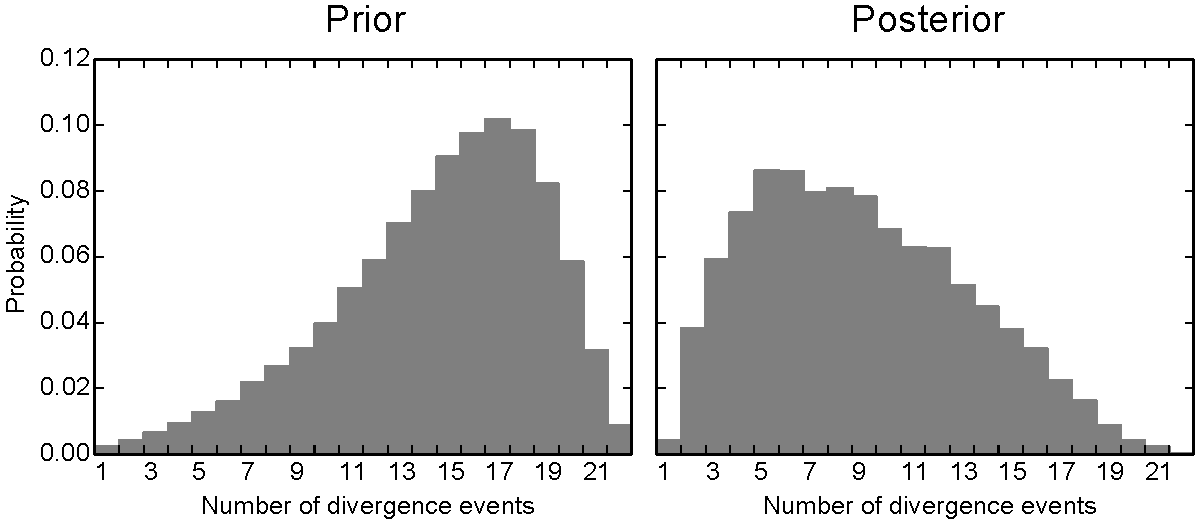
\includegraphics[width=\textwidth]{../../empirical-analyses/plots/philippines-dpp-psi-posterior-prior.pdf}}
    \smallskip
    \centerline{
    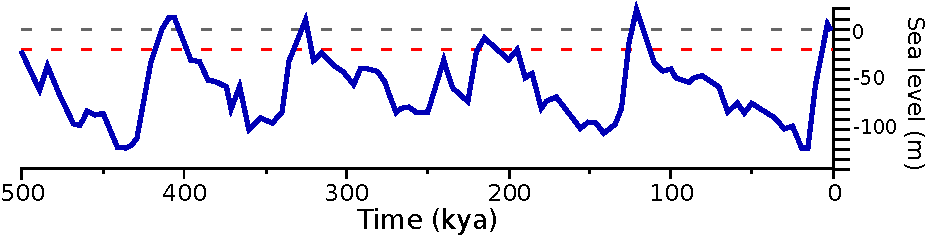
\includegraphics[height=2cm]{../images/sea-level-only.pdf}}
    \barefootnote{\shortfullcite{Oaks2014dpp}}
\end{frame}

\section{Conclusions}

\begin{frame}
    \frametitle{Results}
    \begin{itemize}
        \item<1-> Results consistent with prediction of clustered
            divergences
        \item<2-> Results suggest multiple interglacial periods were important
            drivers of diversification and community assembly across Islands of
            Southeast Asia
        \item<3-> However, there is a lot of uncertainty!
    \end{itemize}
    \barefootnote{\shortfullcite{Oaks2014dpp}}
\end{frame}


\begin{frame}[t]
    \frametitle{Current work: More data}
    \begin{minipage}[t][0.15\textheight][c]{\linewidth}
    \begin{itemize}
        \item<1-> Collecting genomic data from taxa co-distributed across
            Southeast Asian Islands and Mainland
        \item<2-> Preliminary results for 1000 loci from 5 pairs of \emph{Gekko
                mindorensis} populations
    \end{itemize}
    \end{minipage}

    \begin{center}
        \includegraphics<2->[height=5.5cm]{../images/number-of-divs-gekko-mindorensis.pdf}
    \end{center}
\end{frame}

\begin{frame}
    \frametitle{Current work: More power}
    \centerline{
    \includegraphics<1->[height=2cm]{/home/jamie/Dropbox/field-photos/people/mtholder.jpg}
    \hspace{0.6mm}
    \includegraphics<1->[height=2cm]{/home/jamie/Dropbox/field-photos/people/jeet2.jpg}
    \hspace{0.6mm}
    \includegraphics<1->[height=2cm]{/home/jamie/Dropbox/field-photos/people/vladimir.jpg}
    \hspace{0.6mm}
    \includegraphics<1->[height=2cm]{../images/revbayes.png}}

    \begin{itemize}
        \item<1-> Full-likelihood Bayesian implementation
            \begin{itemize}
                \item<2-> Uses all the information in the data
                \item<2-> Applicable to deeper timescales
            \end{itemize}
        \item<3-> Analytically integrate over gene trees
            \footnote{\tiny\shortfullcite{Bryant2012}}
            \begin{itemize}
                \item<4-> Very efficient numerical approximation of posterior 
                \item<4-> Applicable to NGS datasets
            \end{itemize}
    \end{itemize}
\end{frame}


\section{Teaching}

{
\usebackgroundtemplate{\includegraphics[width=\paperwidth]{../images/kane.jpg}}
\begin{frame}[t]
    \vspace{4.5cm}

    \uncover<2->{
    Working with the UW Biology Education Research Group (BERG) \\
    }

    \begin{itemize}
        \item<3-> Designing active-learning modules to teach fundamental concepts
            in evolution and statistics
        \item<4-> Taking an evidence-based approach to the classroom as a lecturer
            for Introductory Biology
    \end{itemize}
\end{frame}
}

\begin{frame}
    \frametitle{Collaborative teaching}
    \centerline{
    
\includegraphics[height=1.5cm]{../images/software-carpentry.pdf}
    }
    Software Carpentry Bootcamp\\

    \begin{uncoverenv}<2->
    \begin{itemize}
        \item Two-day crash course in basic command line and software skills
        \item Taught an international group of biologists how to increase their
            research productivity.
    \end{itemize}
    \end{uncoverenv}
    
    Molecular Evolution Workshops\\

    \begin{uncoverenv}<3->
    \begin{itemize}
        \item Introduce international groups of graduate students, postdocs,
            and faculty to the fundamentals of molecular evolution and
            state-of-the-art software
    \end{itemize}
    \end{uncoverenv}
\end{frame}


\begin{frame}
    \frametitle{Acknowledgments}
    \begin{columns}[t]
        \column{.5\textwidth}
            {\bf Ideas and feedback:}
            \begin{myitemize}
                \item Leach\'{e} Lab
                \item Minin Lab
                \item Holder Lab
                \item Brown Lab/KU Herpetology
                \item Melissa Callahan
            \end{myitemize}
            \smallskip
            {\bf Computation:}\\
            \includegraphics<1->[height={8mm}]{../images/iplant.jpg}
            \hspace{0.5mm}
            \includegraphics<1->[height={8mm}]{../images/kuittc.png}
            \hspace{0.5mm}
            \includegraphics<1->[height={8mm}]{../images/uw.png}\\

        \column{.5\textwidth}
            {\bf Funding:}\\
            \includegraphics<1->[height={8mm}]{../images/nsf.jpg}
            \hspace{0.5mm}
            \includegraphics<1->[height={8mm}]{../images/ngs.jpg}
            \hspace{0.5mm}
            \includegraphics<1->[height={8mm}]{../images/ssb.png}\\

            \smallskip
            {\bf Photo credits:}
            \begin{myitemize}
                \item Rafe Brown, Cam Siler, Jesse Grismer, \& Jake Esselstyn
                \item FMNH Philippine Mammal Website:
                    \begin{myitemize}
                        \item D.S.\ Balete, M.R.M.\ Duya, \& J.\ Holden
                    \end{myitemize}
                \item PhyloPic!
            \end{myitemize}
    \end{columns}
\end{frame}

% \begin{frame}
%     \frametitle{Questions?}    
%     \begin{columns}[c]
%         \column{.5\textwidth}
%         \begin{center}
%             {
%             \Large
%             \href{mailto:joaks1@gmail.com}{\tt joaks1@gmail.com}
%             }
%         \end{center}
%         \column{.5\textwidth}
%             \begin{figure}
%                 \begin{center}
%                 \includegraphics[width=\textwidth]{../images/darwin-tol-copyright-boris-kulikov-2007.jpg}
%                 \caption{\tiny \copyright~2007 Boris Kulikov \href{http://boris-kulikov.blogspot.com/}{boris-kulikov.blogspot.com}}
%                 \end{center}
%             \end{figure}
%     \end{columns}
% \end{frame}

% Extra slides

\begin{frame}[noframenumbering]
    \frametitle{Easy as ABC}
    \centerline{
    \includegraphics<1>[width=\textwidth]{../images/rejection-sampling-observed.pdf}
    \includegraphics<2>[width=\textwidth]{../images/rejection-sampling-tolerance.pdf}
    \includegraphics<3>[width=\textwidth]{../images/rejection-sampling-10.pdf}
    \includegraphics<4>[width=\textwidth]{../images/rejection-sampling-100.pdf}
    \includegraphics<5>[width=\textwidth]{../images/rejection-sampling-200.pdf}
    \includegraphics<6>[width=\textwidth]{../images/rejection-sampling-500.pdf}
    \includegraphics<7>[width=\textwidth]{../images/rejection-sampling-1000.pdf}
    \includegraphics<8>[width=\textwidth]{../images/rejection-sampling-10000.pdf}
    \includegraphics<9>[width=\textwidth]{../images/rejection-sampling-20000.pdf}
    \includegraphics<10>[width=\textwidth]{../images/rejection-sampling-20000-post.pdf}
    }
\end{frame}

\begin{frame}[noframenumbering]
    \frametitle{Causes of bias: Insufficient sampling}
    \begin{itemize}
        \item Models with more parameter space are less densely sampled
        \item Could explain bias toward small models in extreme cases
        \item {\bf Predicts large variance in posterior estimates}
        \begin{itemize}
            \item We explored empirical and simulation-based analyses with
                2, 5, and 10 million prior samples, and estimates were
                very similar
        \end{itemize}
    \end{itemize}
    \smallskip
    \centerline{
    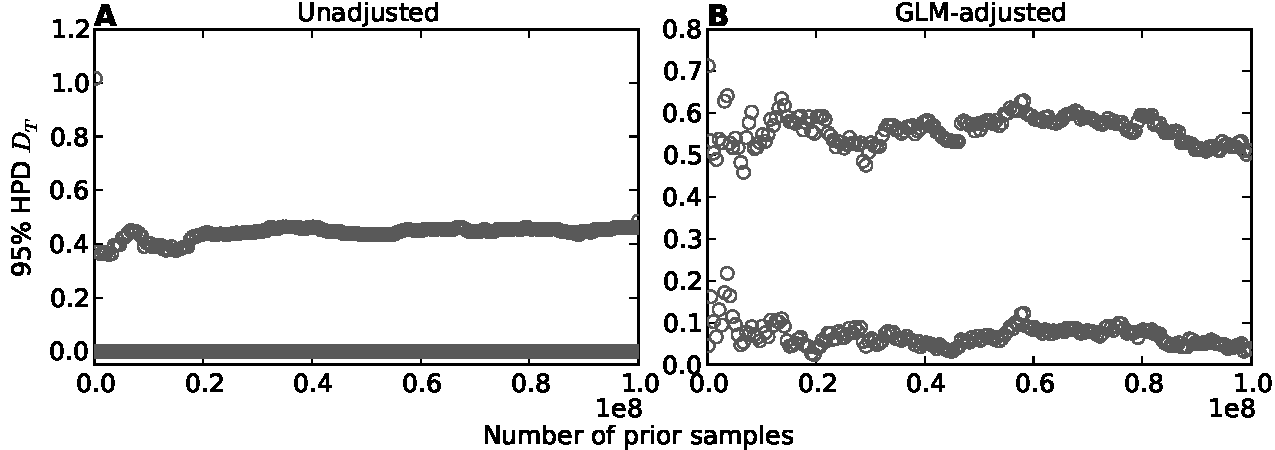
\includegraphics[width=\textwidth]{../images/omega_over_sampling.pdf}}
\end{frame}

\begin{frame}[noframenumbering]
    \frametitle{\dppmsbayes: Simulation results}
    % \vspace{1cm}
        \centerline{
        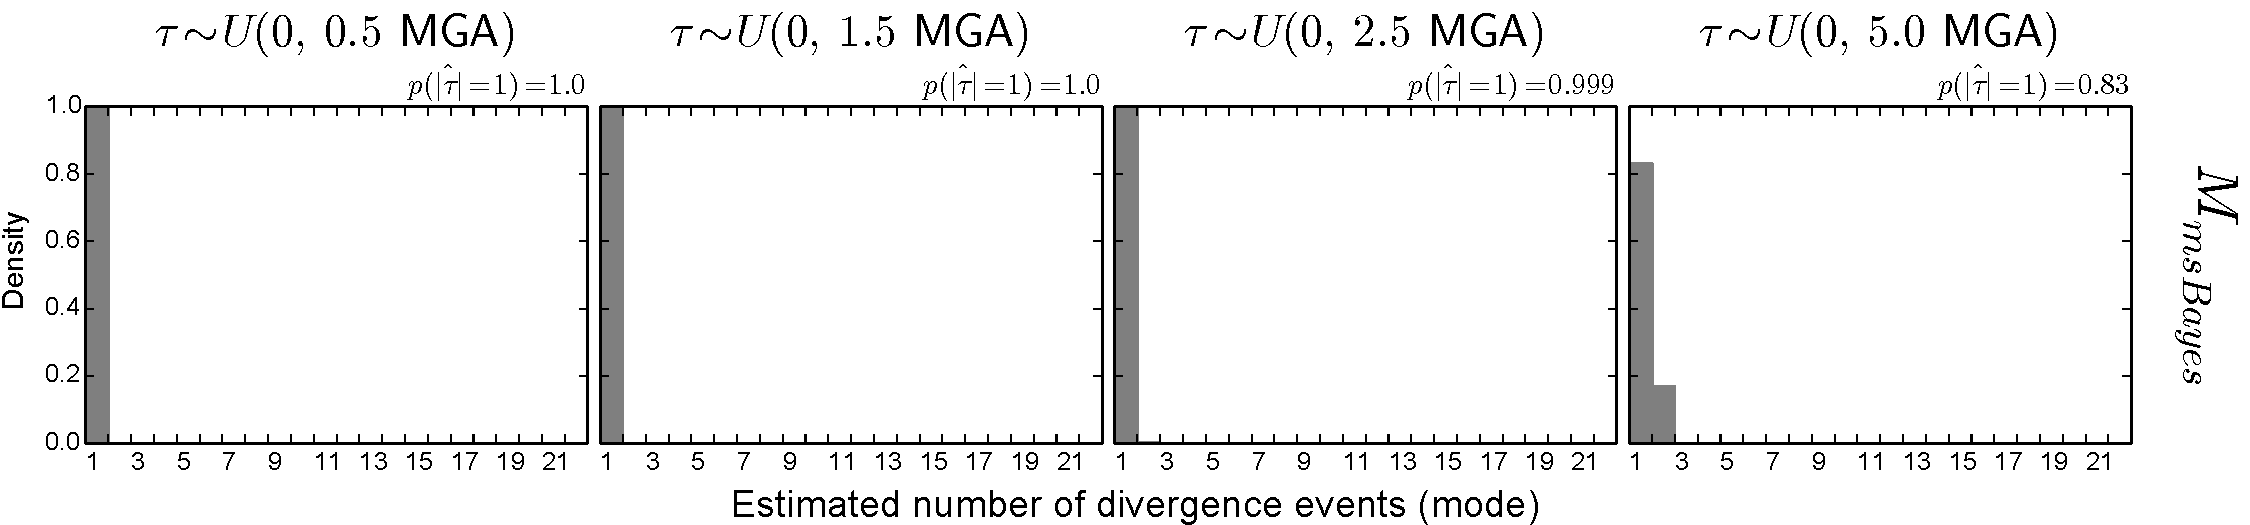
\includegraphics[width=\textwidth]{../images/old_old_power_psi_mode.pdf}}
        \vspace{0mm}
        \centerline{
        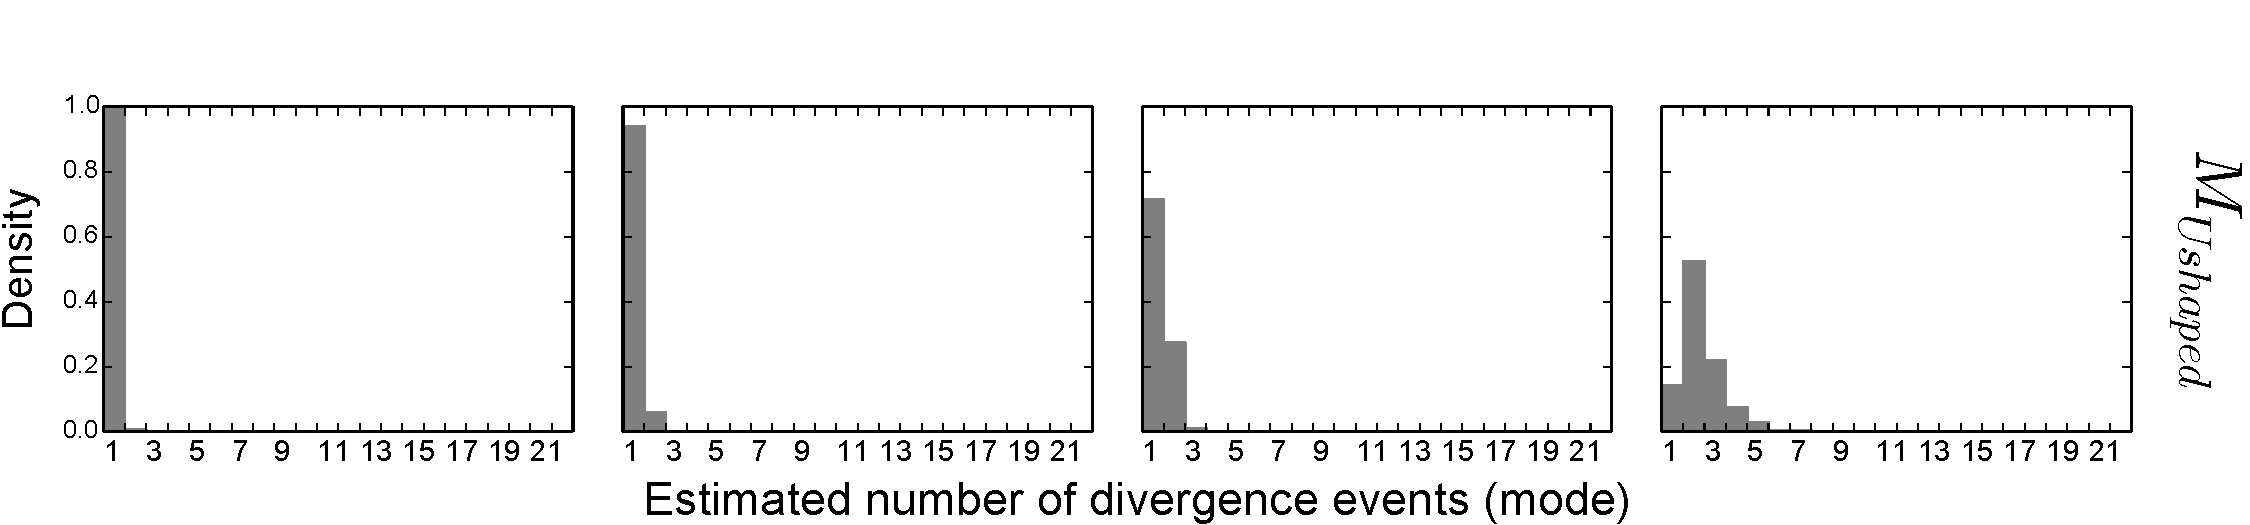
\includegraphics[width=\textwidth]{../images/old_u-shaped_power_psi_mode_headless.pdf}}
        \vspace{0mm}
        \centerline{
        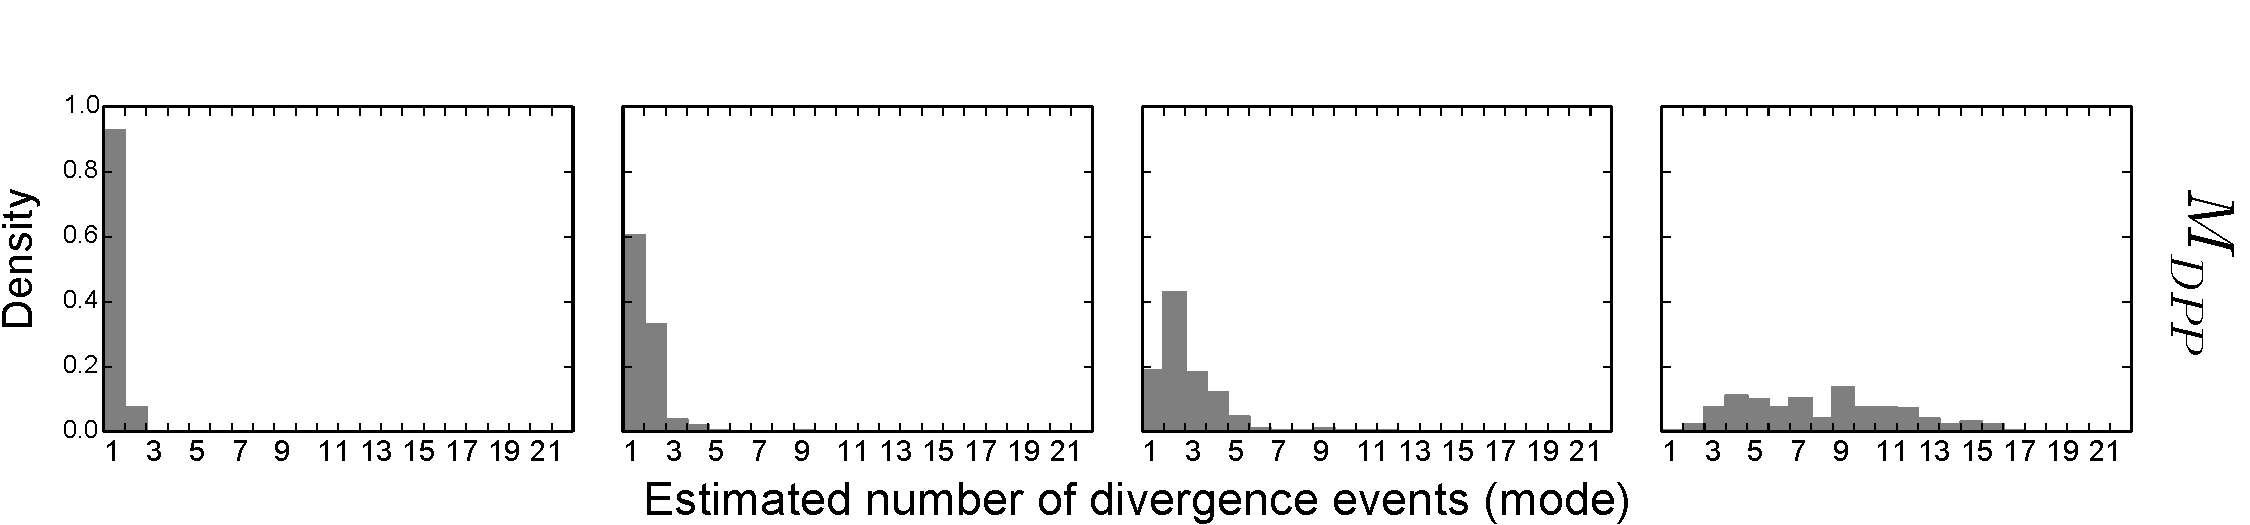
\includegraphics[width=\textwidth]{../images/old_dpp_power_psi_mode_headless.pdf}}
    % \barefootnote{\shortfullcite{Oaks2014dpp}}
\end{frame}

\begin{frame}[noframenumbering]
    \frametitle{\dppmsbayes: Simulation results}
    % \vspace{1cm}
        \centerline{
        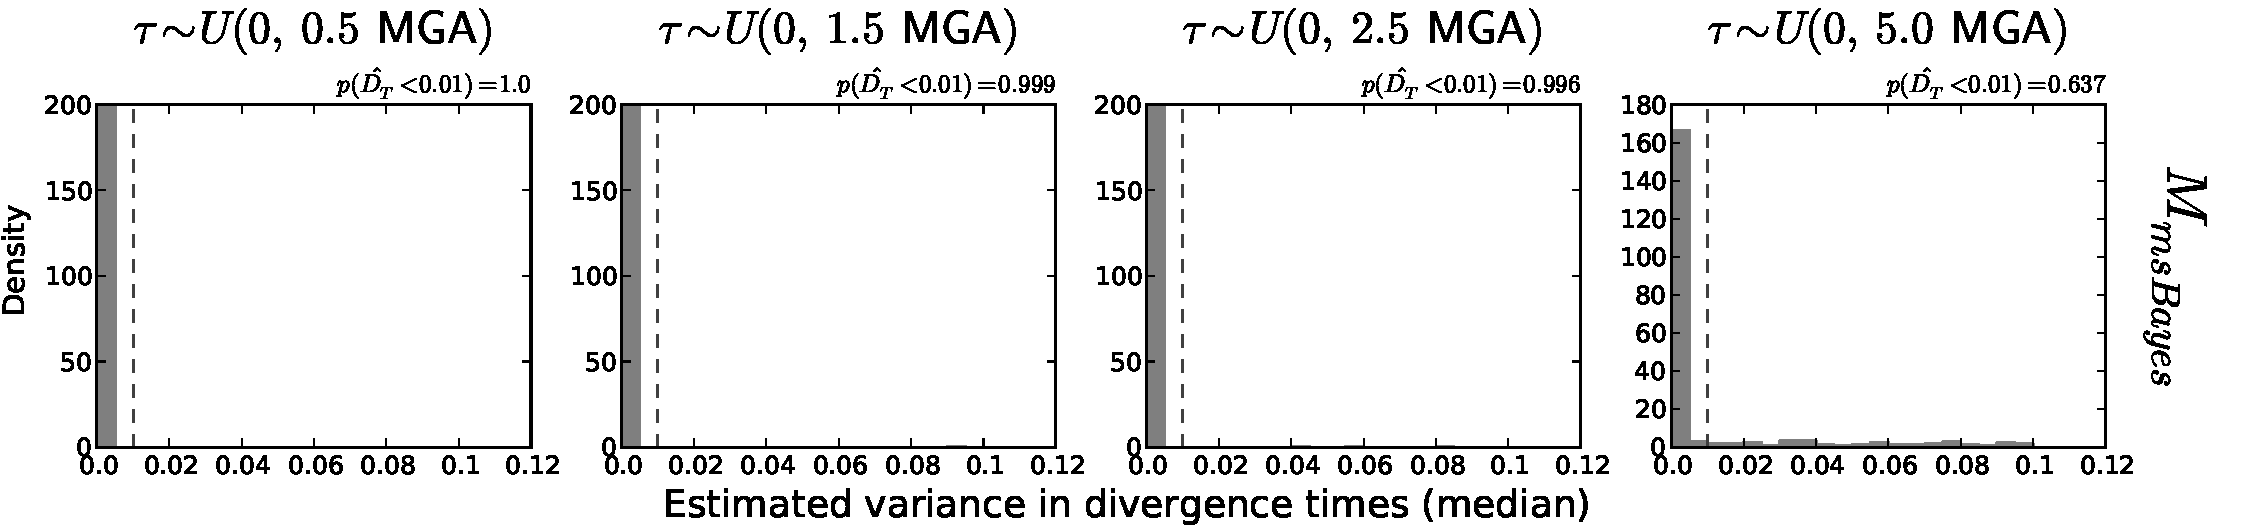
\includegraphics[width=\textwidth]{../images/old_old_power_omega_median.pdf}}
        \vspace{0mm}
        \centerline{
        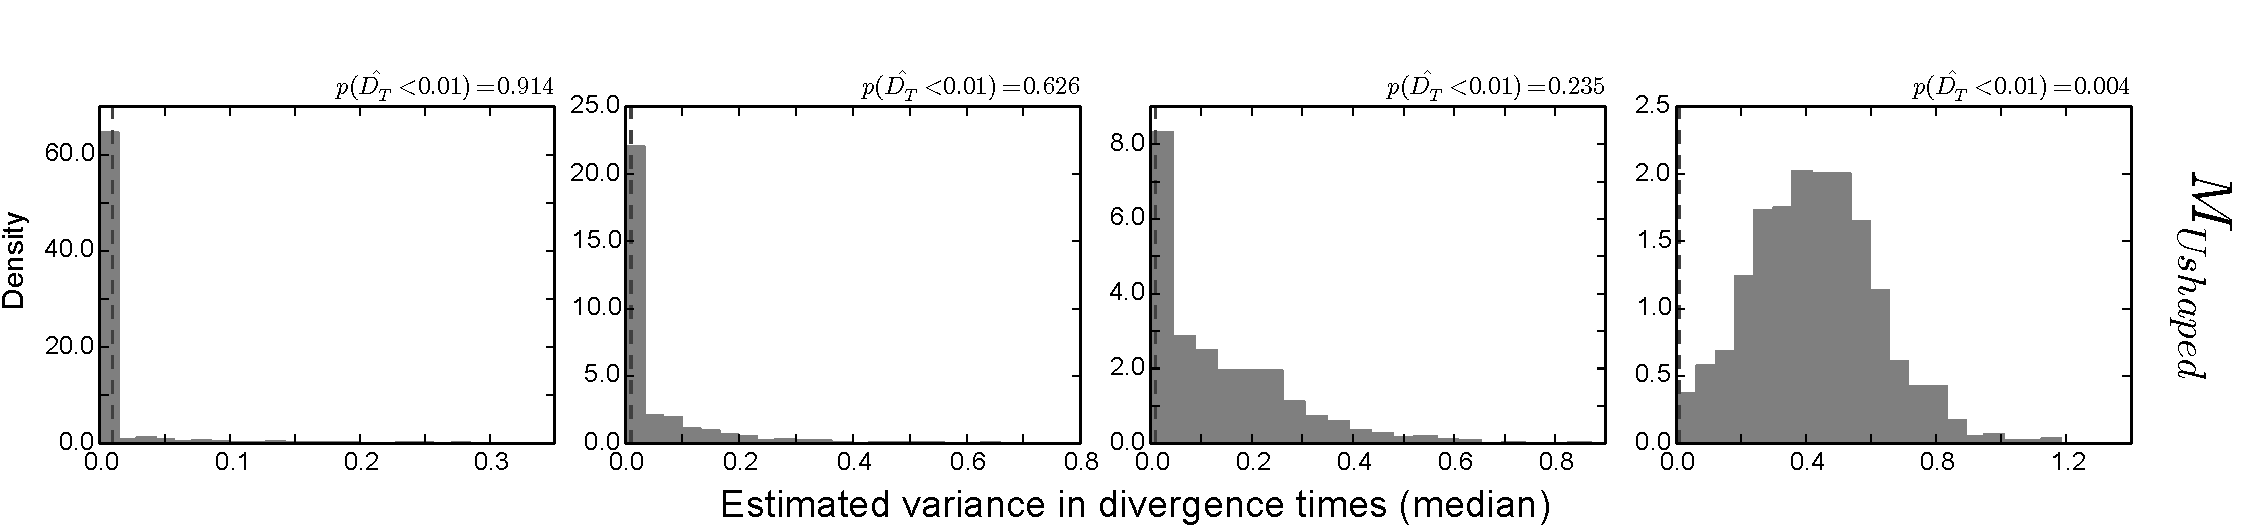
\includegraphics[width=\textwidth]{../images/old_u-shaped_power_omega_median_headless.pdf}}
        \vspace{0mm}
        \centerline{
        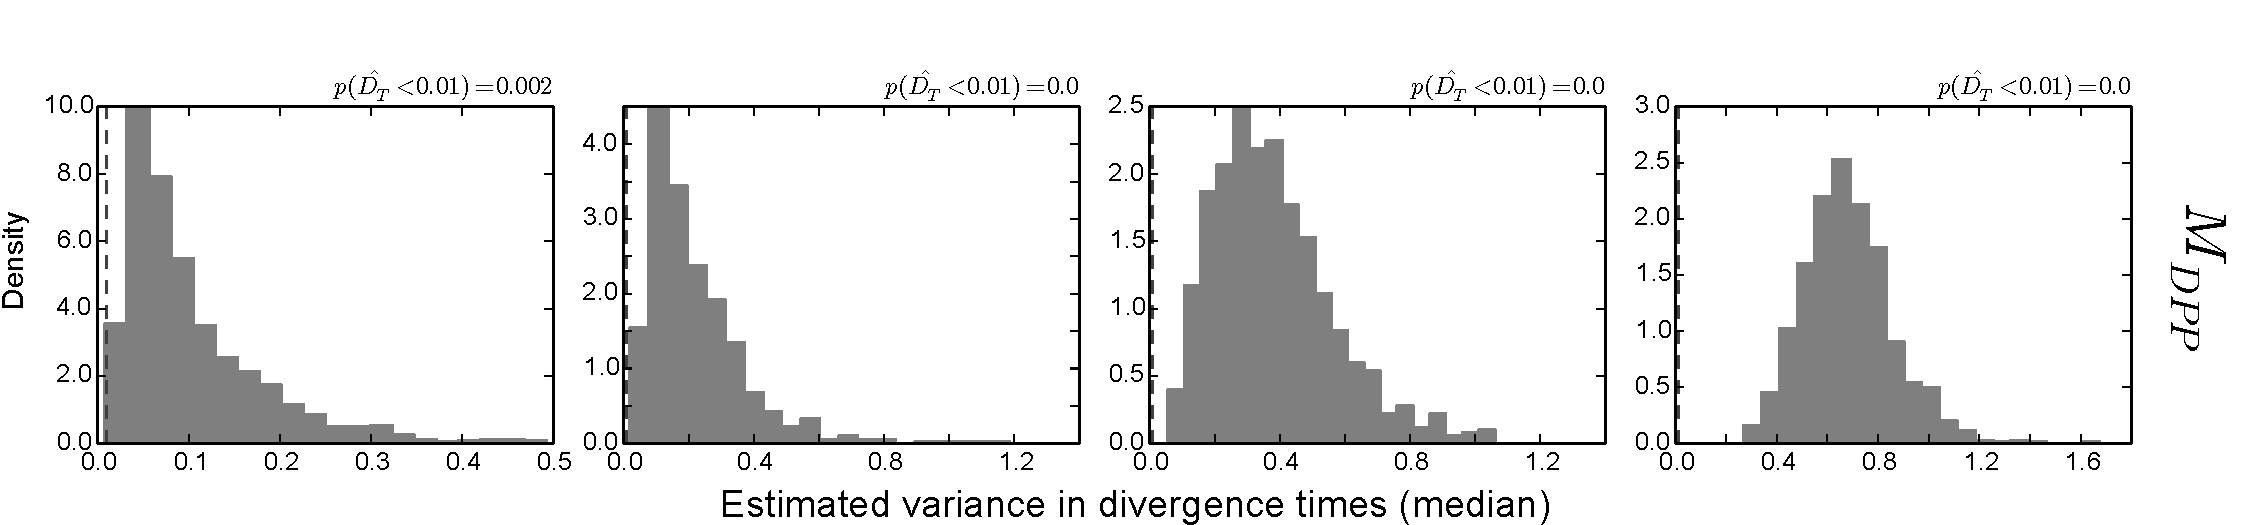
\includegraphics[width=\textwidth]{../images/old_dpp_power_omega_median_headless.pdf}}
    % \barefootnote{\shortfullcite{Oaks2014dpp}}
\end{frame}

\begin{frame}[noframenumbering]
    \frametitle{Empirical results: Philippine diversification}
    \centerline{
    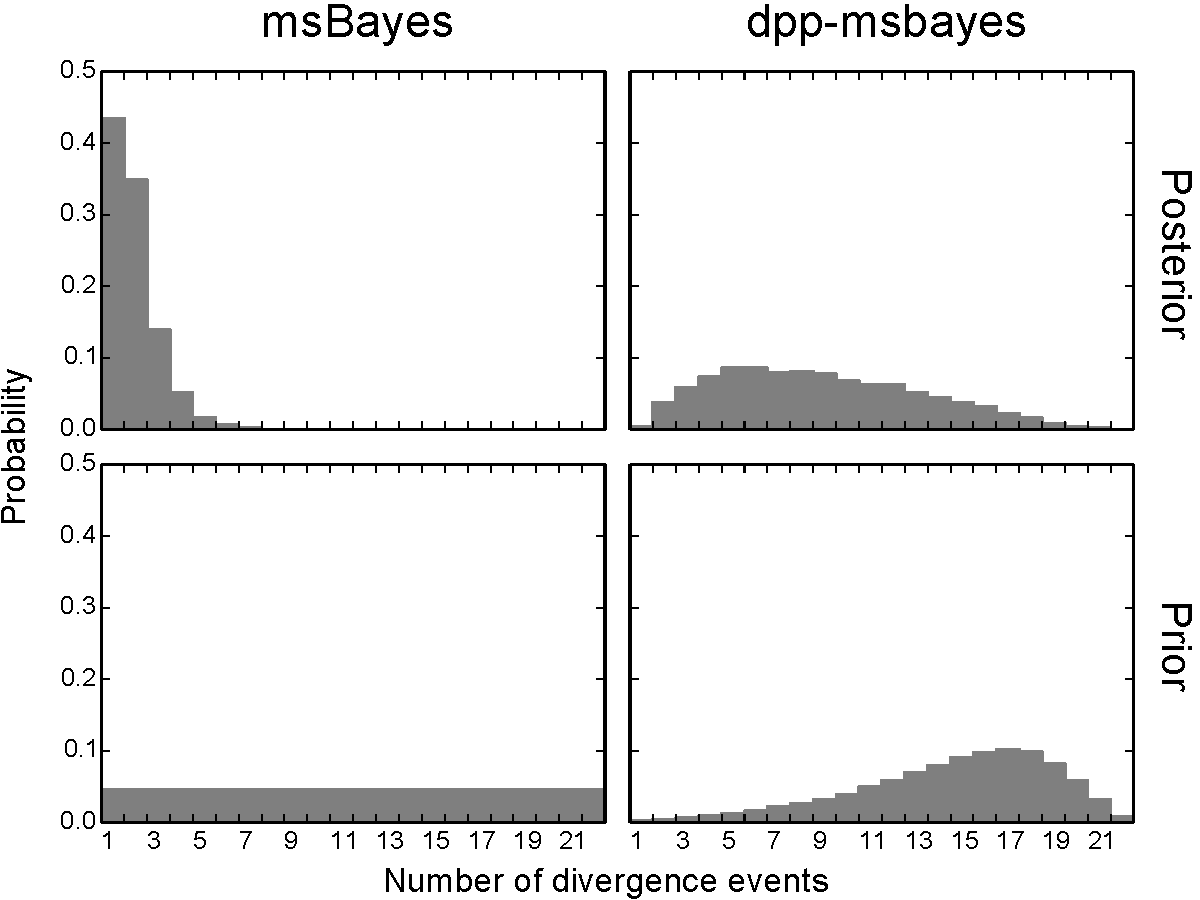
\includegraphics[width=0.8\textwidth]{../../empirical-analyses/plots/philippines-dpp-psi-posterior-old-vs-dpp-with-prior.pdf}}
    \barefootnote{\shortfullcite{Oaks2014dpp}}
\end{frame}


\end{document}

